\documentclass[fleqn,usenatbib,useAMS]{mnras}
\usepackage{amsmath}	% Advanced maths commands
\usepackage{txfonts}
\usepackage[T1]{fontenc}
\usepackage{ae,aecompl}
\usepackage{graphicx,color}	% Including figure files
\usepackage{amssymb}	% Extra maths symbols
\usepackage{amsbsy}
\usepackage[normalem]{ulem}
\usepackage{mathrsfs,bm,xspace}
\newcommand{\bcdot}{\ensuremath{%
  \mathchoice%
   {\mskip\thinmuskip\lower0.2ex\hbox{\scalebox{1.5}{$\cdot$}}\mskip\thinmuskip}}%
   {\mskip\thinmuskip\lower0.2ex\hbox{\scalebox{1.5}{$\cdot$}}\mskip\thinmuskip}%        
   {\lower0.3ex\hbox{\scalebox{1.2}{$\cdot$}}}%  
   {\lower0.3ex\hbox{\scalebox{1.2}{$\cdot$}}}%
}

% --- macros --- %
\newcommand{\Mstream}{{\it M-streaming}\xspace}
\newcommand{\Mflatturb}{{\it M-turbulence}\xspace}
\newcommand{\Mprimary}{{\it M-primaries}\xspace}

\renewcommand{\vec}{\ensuremath{\mathbfit}}
\newcommand{\dd}{\mathrm{d}}
\newcommand{\Vph}{\varv_\mathrm{ph}}
\newcommand{\mug}{\umu G}
\newcommand{\RH}{R_\rmn{RH}}
\newcommand{\bvel}{\ensuremath{\boldsymbol{\varv}}}
\newcommand{\bnabla}{\ensuremath{\boldsymbol{\nabla}}}
\newcommand\eb{\epsilon_\rmn{B}}
\newcommand{\dps}{\displaystyle}
\newcommand{\p}{\rmn{p}}
\newcommand{\kB}{k_{\rmn{B}}}
\newcommand{\eps}{\varepsilon}

%\voffset.6in 

\definecolor{mygreen}{rgb}{0.,0.5,0.}

\title[Origin of Seed Electrons]{Turbulence and Particle Acceleration in Giant Radio Halos: the Origin of Seed Electrons}  

\author[A. Pinzke, S. Peng Oh and C. Pfrommer] 
{Anders Pinzke$^{1,2}$\thanks{apinzke@fysik.su.se (AP); peng@physics.ucsb.edu (SPO); christoph.pfrommer@h-its.org (CP)}, S. Peng Oh$^{3}$ and Christoph Pfrommer$^{4}$\footnotemark[1]\\
$^{1}$The Oskar Klein Centre for Cosmoparticle Physics, Stockholm University, AlbaNova University Center, SE - 106 91
  Stockholm, Sweden\\
$^{2}$Dark Cosmology Center, University of Copenhagen,
  Juliane Maries Vej 30, DK-2100 Copenhagen, Denmark\\
  $^{3}$University of California - Santa Barbara,
  Department of Physics, CA 93106-9530, USA\\
$^{4}$Heidelberg Institute for Theoretical Studies
  (HITS), Schloss-Wolfsbrunnenweg 35, 69118 Heidelberg, Germany}

\begin{document}
\pagerange{\pageref{firstpage}--\pageref{lastpage}} \pubyear{2015}
\maketitle
\label{firstpage}

%\date{\today}

%\pacs{98.65.Cw, 98.70.Sa, 95.85.Bh, 95.30.Qd, 95.30.Cq, 94.05.Lk, 94.05.Pt}

 
\begin{abstract}
  About one third of X-ray-luminous clusters show smooth, unpolarized
  radio emission on $\sim$Mpc scales, known as giant radio halos. One
  promising model for radio halos is Fermi II acceleration of seed
  relativistic electrons by compressible turbulence in the
  intracluster medium (ICM). The origin of these seed electrons has never
  been fully explored. Here, we integrate the Fokker-Planck equation
  of the cosmic ray (CR) electron and proton distributions in
  cosmological simulations of cluster formation, and confront them with radio surface brightness and spectral observations of Coma. For standard
  assumptions, structure formation shocks lead to a seed electron
  population which produces too centrally concentrated radio
  emission. By modifying properties of the CR population (rapid streaming; enhanced CR electron acceleration at shocks) or turbulence (increasing $\eps_{\rm turb}/\eps_{\rm therm}$ with radius), we can match observations, but only at the expense of fine-tuning. We then perform a parameter study. Under naive assumptions, radio properties are exponentially sensitive to the amplitude of turbulence, which is inconsistent with small scatter in scaling relations. This sensitivity can be removed if we relate the acceleration time to the turbulent dissipation time. Their ratio depends only on plasma parameters. In this case, turbulence above a threshold value required to overcome cooling provides a fixed amount of amplification; observations could then potentially constrain the unknown CR seed population. Understanding the small scatter in radio halo scaling relations may prove a rich source of insight on plasma processes in the ICM.   
\end{abstract} 

%% --- keywords --- %
%\begin{keywords}
%  magnetic fields, cosmic rays, radiation mechanisms: non-thermal, elementary
%  particles, galaxies: cluster: general, Galaxy: fundamental parameters
%\end{keywords}
%%\maketitle


% --- section: Introduction --- %
\section{Introduction}
About one third of X-ray-luminous clusters show smooth, unpolarized
radio emission on $\sim$Mpc scales, known as giant radio halos (RHs)
\citep{2014IJMPD..2330007B}. They appear only in disturbed, merging
clusters and the RH luminosity correlates with the X-ray luminosity
\citep{2001A&A...369..441G,2012A&ARv..20...54F} and the Compton
$y$-parameter \citep{2012MNRAS.421L.112B,2013A&A...554A.140P}. The RHs
show that CR electrons and magnetic fields permeate a large volume
fraction of the intra-cluster medium (ICM). The dominant CR source,
given the smoothness and enormous extent of RHs, is thought to be
structure formation shocks \citep{miniati01,pfrommer08}. At the same
time, plasma processes, the origin of magnetic fields and particle
acceleration in a turbulent, high-$\beta$ plasma like the ICM are not
well understood. Radio halos thus provide an incisive probe of
non-thermal processes in the ICM.

There have been two competing models proposed to explain RHs.  The
radio emitting electrons in the ``hadronic model'' are produced in
inelastic (hadronic) CR proton interactions with protons of the
ambient thermal ICM, which generates pions that eventually decay into
electrons and positrons, depending of the charge of the initial pion
(\citealp{1980ApJ...239L..93D,1999APh....12..169B,2001ApJ...562..233M,
  2004A&A...413...17P,2008MNRAS.385.1211P,ensslin11}). CR protons and
heavier nuclei may have been accelerated and injected into the ICM by
structure formation shocks, active galactic nuclei and galactic
winds. However, the strong bimodality that separates X-ray luminous
clusters into radio-active and radio-quite clusters (requiring a
fast switch on/off mechanism of the RH emission) and the very extended
RH emission at low frequencies in Coma (352~MHz) represent a major
challenge to this model class \citep{brunetti12,2014MNRAS.438..124Z}.

The alternative model for RHs is re-energization of seed suprathermal
electrons by Fermi II acceleration when ICM turbulence becomes
transonic during mergers
\citep{1987A&A...182...21S,1993ApJ...406..399G,2001MNRAS.320..365B,
  2004MNRAS.350.1174B,brunetti07,brunetti11,miniati15}. Due
to the short radiative cooling time of high-energy relativistic
electrons, the cluster synchrotron emission quickly fades away after a
merger, which naturally explains the observed bimodality of RHs
\cite[see e.g.][]{2013MNRAS.429.3564D,2014MNRAS.443.3564D}.

However, there is a salient piece missing in the turbulent
reacceleration model. It relies heavily on the assumption of an
abundant, volume-filling population of seed suprathermal electrons;
direct Fermi II acceleration from the thermal pool is precluded by
strong Coulomb losses
\citep{2008ApJ...682..175P,2012ApJ...759..113C}. These seeds are
presumed to be either fossil CR electrons (CRes) accelerated by
diffusive shock acceleration (DSA) during structure formation
\citep{1999ApJ...520..529S}, or secondaries injected by hadronic
interaction of CR protons (CRps) with thermal protons
\citep{brunetti11}.

While analytic estimates have been made, there has been no ab initio
demonstration that structure formation can lead to the required
abundance of seed electrons with the correct spatial and spectral
characteristics. This is a non-trivial requirement: Coulomb cooling in
dense cluster cores is severe, and DSA fossil electrons may not
survive. On the other hand, for secondaries to constitute the seed
population, the CRp population required in the best-studied case of
the Coma cluster must have a very broad and flat (or even slightly
inverted) spatial profile \citep{brunetti12}, in contrast with the
thermal plasma whose energy density declines steeply with radius. In
Fig.~\ref{fig:Edens} we show that such a distribution is not predicted
by cosmological simulations \cite[see
  also][]{pinzke10,2014MNRAS.439.2662V}. If CRps are predominantly
advected with the cluster plasma, their distribution will be peaked
towards the cluster center and shows a similar characteristics as the
thermal plasma. As a consequence, the distribution of secondary
electrons and the resulting radio synchrotron emission is also peaked
since the hadronic reaction is a two-body scattering process. Hence,
the simulated emission falls short of the observed extended and flat
radio profile of the Coma cluster.

\begin{figure}
  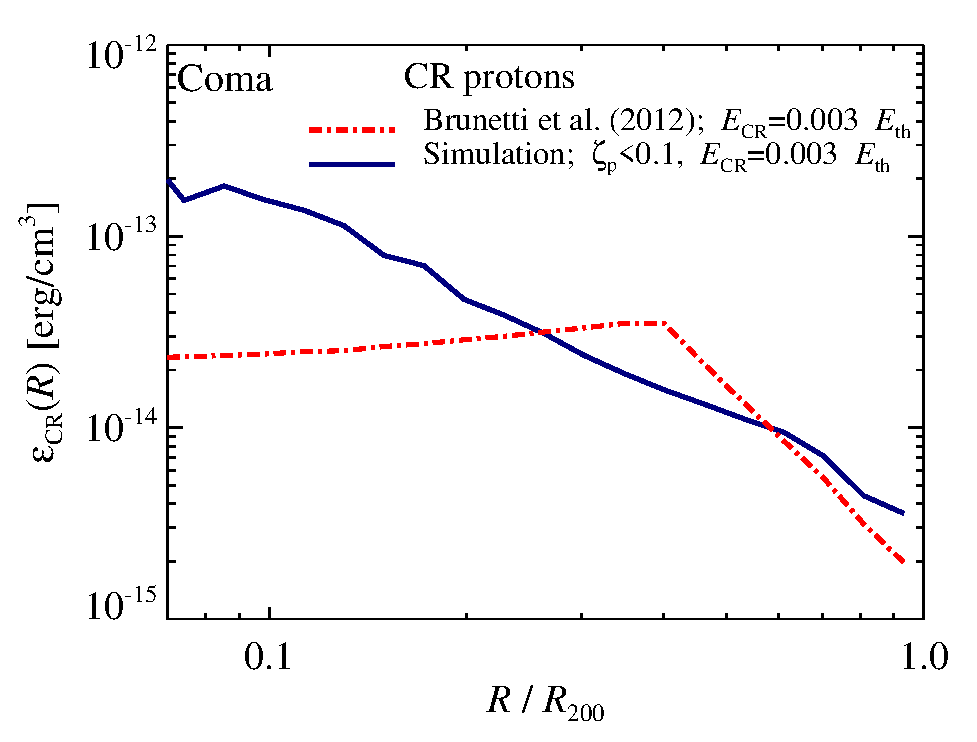
\includegraphics[width=1.0\columnwidth]{fCR.radius.coma.g72a.Rad14.2400p.z0.NL.xKR.eb23.eI067.DII.140.v6.eps}
  \caption{Spatial distribution of CRp energy density in the Coma
    cluster. The red dash-dotted line shows the required distribution
    of seed CRps that generate secondary electrons via proton-proton
    (p-p) collisions required to reproduce Coma radio brightness
    observations after Fermi-II reacceleration \citep{brunetti12}. The
    blue solid line shows the distribution of fossil CRps found in
    cosmological simulations, which disagrees with the required
    profile. To better compare the two models in this figure, we
    normalize the required distribution of CRps by fixing the total
    CRp energy $E_\rmn{CR}$ to 0.3 percent of the total thermal
    energy, consistent with observations
    \citep{2014ApJ...787...18A,2012ApJ...757..123A}.}
  \label{fig:Edens}
\end{figure}

Indeed, arriving at a seed population with the required
characteristics is highly constraining, and has the potential to teach
us much about the origin of CRps/CRes in clusters.  In this work, we
use our hydrodynamical zoom simulations of galaxy clusters in a
cosmological setting to follow the distribution functions of seed
populations for CRps and CRes, and integrate the Fokker-Planck
equation of CR transport along Lagrangian particle trajectories. We
model diffusive shock acceleration at structure formation shocks,
and account for various loss processes of CRs. Utilizing new insights from our recent work on DSA generated
  fossil electrons \citep{pinzke13}, we generate the first
  quantitative calculation of primary and secondary seed electrons

To compare this to observations, we model second-order Fermi acceleration by CR interactions with
magnetised turbulence. However, we assume a simplified and stationary model for magnetic
fields and turbulence. We do not account for the time-varying energy
density in compressible waves, which are thought to be necessary for
the acceleration process \citep{brunetti07,brunetti11}, as the cluster
merger proceeds.  So our approach is orthogonal (and complementary) to
e.g., simulations of \citealp{miniati15} that focus on the
time-dependent compressible turbulence while adopting a simplified
treatment of CR. Our approach of parametrizing turbulence
enables us to vary parameters associated with the spatial profile and the
overall amplitude of compressible waves (that can in principle vary
depending on the details of a particular cluster merger).

In this paper, we explore how the radio surface brightness profile and spectrum of the best known radio halo, Coma, can be used to constrain the underlying properties of the seed cosmic rays and turbulence. We aim to constrain the normalization and spatial profile of these two input ingredients in turbulent reacceleration models. The outline of this paper is as follows. In \S\ref{sect:method}, we outline the basic physics of turbulence reacceleration of cosmic rays which we use. In \S\ref{sec:results}, we use cosmological simulations to generate a seed CR population, and combine it with our parameterized model of turbulence to produce radio surface brightness profiles and spectra of Coma. We find that it is possible to fit the observations using physically motivated modifications of the seed population    
(rapid streaming; enhanced CR electron acceleration at shocks) or turbulence (increasing $\eps_{\rm turb}/\eps_{\rm therm}$ with radius), but only at the expense of fine tuning. In \S\ref{sect:param_comp}, we explore the reason for this fine-tuning, and seek ways to overcome it. We perform a parameter study on spherically symmetric, static models where we vary properties of the seed population and turbulence. We find exponential sensitivity to the amount of turbulent, which can be eliminated if the turbulent acceleration and dissipation time are linked. In this case, turbulence above a threshold value required to overcome cooling provides a fixed amount of amplification; observations could then potentially constrain the unknown CR seed population. We summarize and conclude in \S\ref{sec:conclusions}. 


% --- section: Method --- %
\section{Cosmic ray transport}
\label{sect:method} 

The transport of relativistic electrons and protons across cosmic time
into galaxy clusters is a complex problem that depends on the velocity
field of the gas (and its thermodynamic properties such as density,
temperature, and pressure) as well as non-thermal processes
(turbulence, magnetic fields, fossil CRs). We use high resolution
galaxy cluster simulations to derive the thermal and fossil CR
properties \citep[shock accelerated primary CRes and CRps, as well as
  secondary CRes produced in p-p collisions,
  see][]{2007MNRAS.378..385P,pfrommer08,pinzke10,pinzke13}.


\subsection{Basic equations}
As previously noted, secondaries produced by shock accelerated CRp
have the wrong spatial profile to explain RH observations. Because
they arise from a two body process, they are too centrally
concentrated. They also produce gamma-ray emission in excess of
Fermi-LAT upper limits
\citep{2012ApJ...757..123A,brunetti12,2014ApJ...787...18A}. 

Given a seed population of CRs, we adopt essentially the same set of
plasma physics assumptions as the reacceleration model for RHs
\citep{brunetti07,brunetti11}. We solve the isotropic, gyro-phase
averaged Fokker-Planck equation (via a Crank-Nicholson scheme) for the
time evolution of the CRe distribution in the Lagrangian frame
\citep{brunetti07,brunetti11}:
\begin{eqnarray}
{{d f_{\rmn{e}}(p,t)}\over{d t}} &\!=&
\frac{\partial}{\partial p}
\left\{
f_{\rmn{e}}(p,t)\left[
\left|\frac{dp}{dt}\right|_{\rm Coul} 
+ \frac{p}{3}\left(\bnabla\bcdot \bvel\right)
+ \left|\frac{dp}{dt}\right|_{\rm rad}\right.\right.
\nonumber\\
&-& \left.\left.{1\over{p^2}}{{\partial }\over{\partial p}}\left(p^2 D_{\rm pp}\right) 
\right]\right\} - \left(\bnabla\bcdot \bvel\right) f_{\rmn{e}}(p,t)
\nonumber\\
&+& {{\partial^2 }\over{\partial p^2}}
\left[
D_{\rm pp} f_{\rmn{e}}(p,t) \right]+ Q_{\rmn{e}}\left[p,t;f_{\rmn{p}}(p,t)\right]   \, .
\label{elettroni}
\end{eqnarray}
Here $f_{\rmn{e}}$ is the one-dimensional distribution in position $x$
(suppressed for clarity), momentum $p$ and time $t$ (which is
normalized such that the number density is given by
$n_{\rmn{e}}(t)=\int d p f_{\rmn{e}}(p,t)$), $d/dt=\partial/\partial
t+\bvel\bcdot\bnabla$ is the Lagrangian derivative, $\bvel$ is the gas
velocity, $|dp/dt|$ represents Coulomb
\citep[Coul,][]{1972Phy....60..145G} and radiative
\citep[rad,][]{1979rpa..book.....R} losses, respectively,
\begin{eqnarray}
   \left|\frac{dp}{dt}\right|_{\rm Coul} &=& \frac{3\,\sigma_\rmn{T}\,n_e\,c}{2\, \beta^2}
  \left[\ln\left(\frac{m_e c^2 \beta \sqrt{\gamma-1}}{\hbar\,\omega_\rmn{plasma}}\right)\right.\nonumber \\
    &-&\ln(2)\left(\frac{\beta^2}{2}+\frac{1}{\gamma}\right)+\frac{1}{2}+
    \left.\left(\frac{\gamma-1}{4\gamma}\right)^2\right]\,, \\
  \left|\frac{dp}{dt}\right|_{\rm rad~} &=& \frac{4}{3}\frac{\sigma_\rmn{T}}{m_ec}\,
  \frac{p^2}{\beta}\,\left[1+\left(\frac{B}{B_\rmn{CMB}}\right)^2\right]\,.
\end{eqnarray}
Here $\beta = p/\sqrt{1+p^2}$ is the dimensionless velocity of CRs,
$\gamma=\sqrt{1+p^2}$ is the Lorentz factor of CRs,
$\omega_\rmn{plasma} = \sqrt{4\pi e^2 n_e / m_e}$ is the plasma
frequency, $n_e$ is the number density of free electrons, and
$\sigma_\rmn{T}= 8\pi e^4/3(m_e c^2)^2$ is the Thomson cross
section. The {\it rms} magnetic field strength is denoted by $B$ and
the equivalent field strength of the cosmic-microwave background is
given by $B_\rmn{CMB} = 3.24 (1 + z)^2\mu\rmn{G}$, where $z$ denotes
the redshift. In the peripheral cluster regions, where $B \ll
B_\rmn{CMB}$, the CRes loose virtually all their energy by means of
inverse Compton emission. $D_{\rm pp}$ is the momentum space diffusion
coefficient (see \S\ref{sec:reacc}), and
$Q_{\rmn{e}}$ denotes the injection rate of primary and secondary
electrons in the ICM (see Sect.~\ref{sec:cosmo_sim}). The first term
containing the expression $\bnabla\bcdot \bvel$ represents Fermi-I
acceleration and the second term of this form describes adiabatic
gains and losses.

During post-processing of our Coma-like cluster simulation, we solve
the Fokker-Planck equation over a redshift interval from $z=5$ to
0. The simulated cluster undergoes a major merger over the last
1-2~Gyrs that is thought to inject large turbulent eddies. As is commonly assumed \citep{brunetti07,brunetti11,2004ApJ...614..757Y,2013ApJ...771..131B}
we assume that about one Gyr after core passage the fields have
decayed down to the smallest scales $k_{\rm cut}$, and the radio halo turns on
shortly after. We choose this simulation snapshot to analyze. We are not very sensitive to this assumption, since the thermal and CR quantities are very similar a few
100 Myrs before and after z = 0, where we have chosen to evaluate the
simulations. In all our
calculations we assume that turbulent reacceleration efficiently
accelerates particles for $\tau{\rm cl} \sim 650$ Myrs (which is roughly the cascade
time on which turbulence is damped) and that during this turbulent
phase CR streaming and spatial diffusion can be neglected. In \S\ref{sect:self-limiting}, we explore sensitivity to the last assumption.


Thus far, we have ignore CR transport. However, if CRps stream in the ICM, then their spatial profile could
potentially flatten sufficiently \citep{ensslin11,wiener13}. This
scenario is very attractive: it generates seed electrons with the
right spatial footprint, and by removing CRps from the core, obeys
gamma-ray constraints. Turbulence plays two opposing roles:
Alfv{\'e}nic turbulence damps waves generated by the CR streaming
instability \citep{yan02,farmer04}, thus reducing self-confinement;
but compressible fast modes scatter CRs directly. Turbulent damping is
still efficient for highly subsonic conditions \citep{wiener13}, while
we assume compressible fast modes to only provide effective spatial
confinement during the periods of transonic, highly super-Alfv{\'e}nic
($M_{\rm A} \sim 5$) turbulence associated with mergers. Thus, CRs can
stream out when the cluster is kinematically quiescent. Furthermore,
even Alfv{\'e}nic streaming timescales are relatively short
\cite[$\sim 0.1-0.5$ Gyr;][]{wiener13} compared to the timescale on
which the CRp population is built up. Based on these findings, we
adopt a toy model for our \Mstream scenario in which CR streaming
instantaneously produces flat CRp profiles. We assume that CRs cannot stream significantly past
perpendicular $B$-fields at the accretion shock, so that the total
number of CRs is conserved within the virial radius during the
streaming process.
In all our calculations we assume that turbulent reacceleration
efficiently accelerates particles for $\tau_\rmn{cl}\sim650$~Myrs
(which is roughly the cascade time on which turbulence is damped) and
that during this turbulent phase CR streaming and spatial diffusion
can be neglected. 

The time evolution of the spectral energy distribution of CRps,
$f_{\rmn{p}}$, is similarly given by:
\begin{eqnarray}
\lefteqn{
  {{d f_{\rmn{p}}(p,t)}\over{d t}} =
  {{\partial }\over{\partial p}}
  \left\{
  f_{\rmn{p}}(p,t)\left[ \left|{{dp}\over{dt}}\right|_{\rm Coul}
    + \frac{p}{3}\bnabla\bcdot \left(\bvel+\bvel_{\rmn{st}}\right)\right.\right.}
\nonumber\\
&&-\left.\left. {1\over{p^2}}{{\partial }\over{\partial p}}\left(p^2 D_{\rm pp}\right)
\right]\right\} - f_{\rmn{p}}(p,t) \bnabla\bcdot \left(\bvel+\bvel_{\rmn{st}}\right) 
- \bvel_{\rmn{st}}\bcdot\bnabla f_{\rmn{p}}(p,t)
\nonumber\\
&&+\,\,\, {{\partial^2 }\over{\partial p^2}}
\left[ D_{\rm pp} f_{\rmn{p}}(p,t) \right] - {{f_{\rmn{p}}(p,t)}\over{\tau_{\rm had}(p)}}
+ Q_{\rmn{p}}(p,t)\, ,
\label{eq:FP_p}
\end{eqnarray}
where $\bvel_{\rmn{st}}=-\varv_{\rmn{A}}\bnabla f_{\rmn{p}}/|\bnabla
f_{\rmn{p}}|$ is the streaming velocity in the isotropic transport
approximation, $\varv_{\rmn{A}}$ is the Alfv\'en speed,
and $Q_{\rmn{p}}(p,t)$ denotes the injection rate of shock accelerated
CRps as a function of momentum $p$ and time $t$ (see
Sect.~\ref{sec:cosmo_sim}). The timescale of
hadronic losses that produce pions via CRp collisions with thermal
protons of the ICM is given by 
\begin{eqnarray}
  \tau_{\rm had} = \left[c\,n_\rmn{th}\,\sigma^{+/-,0}(p)\right]^{-1}\,,
\end{eqnarray}
where we use the cross-section, $\sigma^{+/-,0}(p)$, given by the
fitting formula in \citep{1986ApJ...307...47D}.

\subsection{Turbulent Reacceleration}
\label{sec:reacc}

In turbulent reacceleration, particles gain energy via Fermi II acceleration. Wave-particle energy exchange takes place via transit time damping \citep{brunetti07,brunetti11}. The
TTD resonance requires the wave frequency to obey the resonance
condition, $\omega=k_\parallel\varv_\parallel$, where $k_\parallel$
and $\varv_\parallel$ are the parallel (projected along the magnetic
field) wavenumber of the compressible mode and particle velocity, respectively. This implies
that the particle transit time across the confining wave region
matches the wave period,
$\lambda_{\parallel}/\varv_{\parallel}=\tau_{\rmn{wave}}$ (hence the moniker, 'transit time damping'). Note that the CRs'
gyroradius does not enter the resonance condition. Hence the CRs that
are in resonance with compressible waves experience Fermi-II
acceleration irrespectively of the length scale of the perturbation.

However, the resonance changes the component of the particle momentum
parallel to the mean magnetic field, which over time leads to
increasing anisotropy in the particle distribution that decreases the
efficiency of reacceleration with time. As in \citet{brunetti11}, we
assume that there exists a mechanism---such as the firehose
instability---that isotropizes the CR distribution function at the
gyroscale and on the reacceleration time scale, which ensures
sustained efficient reacceleration with time.

All of the physics of turbulent reacceleration is effectively encapsulated in the diffusion coefficient \citep{brunetti07}, which can be rewritten as \citep{miniati15}:
\begin{equation}
D_{\rm pp}(p) = \frac{ p^{2} \pi I_{\theta}(c_{s}/c)}{8 c} \langle k \rangle_{\mathcal{W}} \langle (\delta \varv_{\rm c})^{2} \rangle
\label{eqn:diffusion}
\end{equation}
where $I_{\theta}$ averages interaction rates over the CR pitch angle $\theta$; $I_{\theta} \approx 5$ for ICM conditions, and
\begin{equation}
\langle k \rangle_{\mathcal{W}} = \frac{1}{\langle (\delta \varv_{\rm c})^{2} \rangle} \int_{k_{\rm L}}^{k_{\rm cut}} dk \, k \, \mathcal{W}(k) \approx \frac{s-1}{2-s} k_{\rm L} \left( \frac{k_{\rm cut}}{k_{\rm L}} \right)^{2-s} 
\label{eqn:k_W} 
\end{equation}
is an energy-averaged wavenumber, $k_{\rm L}, k_{\rm cut}$ are the wavenumbers associated with the outer scale and the cutoff scale respectively, and we have assumed a total energy spectrum (both kinetic and potential energy, where the two are assumed to be in equipartition \citep{sarkar11}): 
\begin{equation}
\mathcal{W}(k) = \frac{(s-1) \langle (\delta \varv_{\rm c})^{2} \rangle}{k_{\rm L}} \left( \frac{k}{k_{\rm L}} \right)^{-s} 
\label{eqn:Wk}
\end{equation}
which defines the normalization $\langle (\delta \varv_{\rm c})^{2} \rangle$ (the subscript 'c' emphasizes that we specialize to compressive modes). Intuitively, we can understand the form of the the diffusion coefficient from the fact that for second-order Fermi acceleration, $\dot{p} \sim \Delta p/\tau \sim p\,\langle k c \rangle_{\mathcal{W}} (\delta \varv_{\rm c}/c)^{2}$, where $\tau^{-1} \sim \langle k c \rangle_{\mathcal{W}}$ is the energy averaged wave-particle interaction rate, and $\Delta p \sim p (\delta \varv_{\rm c}/c)^{2}$ is the typical momentum change during wave particle scattering. Thus: 
\begin{equation}
D_{\rm pp} \sim p \dot{p} \sim p^{2} \langle k c \rangle_{\mathcal{W}} \left( \frac{\delta \varv_{\rm c}}{c} \right)^{2}. 
\end{equation}

Equations \ref{eqn:diffusion} and \ref{eqn:Wk} make the important aspects of turbulence clear: the energy in compressive modes $\langle (\delta \varv_{\rm c})^{2} \rangle$, the inner and outer scale ($k_{\rm cut}$ and $k_{\rm L}$), and the slope of the energy spectrum $s$. All of these can vary spatially and temporally. 

We adopt a Kraichnan spectrum ($s=3/2$) for the fast modes, as seen in simulations \citep{cho03}. This can also be written as: 
\begin{equation}
  \label{eq:Wk}
  \mathcal{W}(k) =
\sqrt{2/7\,I_0\,\rho\,\langle \Vph \rangle}\,k^{-3/2},
\end{equation}
where $I_{\rm 0}$ is the volumetric injection rate of turbulence (which is assumed to be constant), $\varv_{\rm ph}\approx c_{\rm s}$ is the phase speed of waves. It is important to realize that this only applies at small scales, which turbulence is MHD. At large scales, turbulent motions are subsonic (${\mathcal M}_{\rm s} \sim 0.2-0.5$) but super-Alfv{\'e}nic (${\mathcal M}_{\rm A} \sim 5$). Thus, except in the case where motions are transonic and weak shocks become important, motions are fundamentally hydrodynamic and turbulence follows a Kolmogorov ($s=5/3$) spectrum. However, while the turbulent energy density $U_{\rm t} \propto l^{2/3}$ decreases at small scales, the magnetic energy density is scale-independent. Thus, at some scale $l_{\rm A} \sim l_0 {\mathcal M}_{\rm A}^{-3}$, where $U_{\rm turb} \sim U_{B}$, the magnetic field becomes dynamically important, and turbulence transitions to the MHD regime. The cutoff scale in equation \ref{eqn:Wk} can be computed by setting the turbulent cascade rate for fast modes to the transit time damping rate on thermal electrons. This yields \citep{brunetti07,miniati15}:
\begin{equation}
k_{\rm c} \approx A k_{\rm outer} \frac{\langle \varv_{\rm outer}^{2}\rangle^{2}}{c_{\rm s}^{4}}
\label{eqn:k_c} 
\end{equation}
where $A \approx 11 000$. This gives $2\upi/k_\rmn{cut}\sim 0.1-1$~kpc in the ICM. This constitutes an
effective mean free path for CRs, unless plasma instabilities can
mediate interactions between turbulence and particles on smaller
scales \citep{brunetti11}, a possibility we discuss in \S\ref{sect:self-limiting}. Another possibility is that compressible modes dissipate in weak shocks, resulting in Burgers' turbulence $s=2$ \citep{kowal10,porter15,miniati15}. If Burgers turbulence dominates, then particle acceleration rates are too slow in the face of cooling processes to explain radio halos \citep{miniati15}, and an alternative model for radio halos is required. 

The spatial profile of injected turbulence depends on the details of the
merger such as time during the merger, the impact parameter, the
merger mass ratio, and the degree of cluster anisotropy
\citep{miniati15}. We parametrize these uncertainties and
assume that volumetric injection rate of turbulent energy,
$I_0\propto \eps_\rmn{th}^{\alpha_\rmn{tu}}$, and determine the
normalization by requiring that the turbulent energy in compressible
modes $E_\rmn{turb}=\int \int \mathcal{W}(k) \rmn{d}k \rmn{d}V =
X_\rmn{tu} E_\rmn{th}$, where $E_\rmn{th}$ is the total thermal
energy. Given these definitions, one can show that: 
\begin{equation}
  \label{eq:Dpp_scaling}
  D_{\rm pp}\propto \frac{I_0}{\rho c_{\rmn{s}}} \propto 
X_\rmn{tu}^2k_{\rm L} \eps_\rmn{th}^{\alpha_\rmn{tu}-1}\sqrt{T}\,.
\end{equation}

What is a typical energy density in compressive fast modes? The total turbulent energy is typically $\sim 15-70\%$ of the thermal energy in a cluster \citep{vazza11}; it rises rapidly during a merger. The compressible component is $\sim 20-40\%$ of the total turbulent energy, and shows more rapid temporal variations compared to the compressible component \citep{2013ApJ...771..131B,miniati15}. Note the compressible component in cluster simulations is much larger than that seem in stirring box simulations with similar Mach numbers \citep{kowal10,lynn14}. This is likely due to the compressive nature of turbulent driving (transonic infall and merger), whereas idealized simulations tend to use incompressible solenoidal driving and allow compressive fluctuations to develop on their own. Overall, we adopt a compressive energy density which is $X_{\rm tu} \sim 0.2$ of the thermal energy as a baseline estimate. 

The important effects are best summarized in terms of the acceleration time: 
\begin{equation}
\tau_{\rm D}= \frac{p^{2}}{4 D_{\rm pp}}
\end{equation}
which is momentum independent. This should be compared against the lifetime of turbulence, $\tau_{\rm cl}$, and the cooling time $\tau_{\rm cool}$. In Table~\ref{tab:timescales}, we show both the thermal quantities and the
timescales for CR cooling and (re)acceleration for three different
spatial regions of the RH. The densities \citep{1992A&A...259L..31B} and temperatures \citep{2009ApJ...696.1886B,2001A&A...365L..67A} are derived from X-ray observations. To calculate synchrotron cooling times, we use B-fields derived from Faraday rotation measurements \citep{bonafede10}. To calculate the acceleration time, we need to assume an outer scale. We assume an injection scale $k_{\rm L}=2\pi/\lambda_{\rm L}$, where $\lambda_{\rm L} = 100$ kpc, which were assumptions adopted in previous work \citep{2006MNRAS.366.1437S,brunetti07, brunetti11}. This lengthscale corresponds to an eddy turnover time on the outer scale of $\varv_{L} k_{\rm L}^{-1} \sim 1.2$Gyr if $\varv_{\rm L} \sim 500 {\rm km \, s^{-1}}$, as is characteristic of a merger. Note that hydrodynamical simulations of clusters have sometimes found larger $\lambda_{\rm L}$, in some cases comparable to the size of the cluster \citep{vazza11,miniati15}. This choice is degenerate with $X_{\rm tu}$; in \S\ref{sect:self-limiting} we argue that $k_{\rm A}$ is a more appropriate choice, but also find that when the decay time is appropriately scaled, we are relatively insensitive to the choice of $k_{\rm L}$. We present $\tau_{\rm D}$ for 3 different models, which we discuss in the next section. The reacceleration timescale
$\tau_{\rm D}$ is similar between our three models, where the
difference comes from turbulent profile parameterized with
$\alpha_\rmn{tu}$. This implies that even small differences in the
turbulent profile could impact the seed CRs significantly. Finally, we adopt an duration of acceleration $\tau_{\rm cl} = 650$ Myr, in line with previous assumptions \citep{brunetti07}, roughly corresponding to the turbulent decay time. 
\begin{table}
  \caption{Thermal quantities and timescales for different spatial
    regions in a Coma like cluster.}
\begin{tabular}{l c  c c}
\hline
\hline
& & spatial regions & \\
 & $0.1\,\RH^{(2)}$ & $0.3\,\RH^{(2)}$ & $\RH^{(2)}$   \\
\hline
thermal quantities$^{(1)}$ & & & \\
$\rho$ [$10^{-27}$ g cm$^{-3}$] & 3.0 & 1.6 & 0.15 \\
$T$ [$10^{8}$ K] & 1.4 & 1.0 & 0.58 \\
\hline
timescales$^{(1)}$ & & & \\
$\tau_\rmn{D}$(\Mprimary)$^{(3)}$ [Gyr] & 0.45 & 0.44 & 0.39 \\
$\tau_\rmn{D}$(\Mstream)$^{(3)}$  [Gyr] & 0.50 & 0.47 & 0.34 \\
$\tau_\rmn{D}$(\Mflatturb)$^{(3)}$  [Gyr] & 0.69 & 0.56 & 0.27 \\
$\tau_\rmn{IC/sync}(P=10^4\,m_ec)^{(4)}$ [Gyr] & 0.11 & 0.15 & 0.22 \\
$\tau_\rmn{had}(P=100\,m_pc)^{(5)}$ [Gyr] & 2.4 & 4.5 & 47 \\
$\tau_\rmn{Coul}(P=\,m_ec)^{(6)}$  [Gyr] & 0.0092 & 0.017 & 0.17 \\
\hline
\end{tabular}
\begin{quote}
 Notes: \\ 
 (1) Median quantities from our simulated post-merging cluster g72a derived 
 during last 300~Myrs in time. \\
 (2) Radius of the giant radio halo in Coma where $\RH\approx0.6\,R_{200}$.\\
 (3) Fermi-II reacceleration for both electrons and protons at all energies.\\
 (4) Inverse Compton and synchrotron cooling for electrons.\\
 (5) Catastrophic losses for protons.\\
 (6) Coulomb cooling for electrons (protons factor $m_e/m_p$ smaller).\\
 \label{tab:timescales}
  \end{quote}
\end{table} 


% --- section: Simulation Results and discussion --- %
\section{Cosmological simulations}
\label{sec:results}

In this section, we solve the Fokker-Planck equation for CR transport
on Lagrangian particle trajectories through cosmic history. We then use our parameterized model of turbulence to apply turbulence re-acceleration, and compare radio halo profiles against observations of the Coma cluster. Our philosophy to is make assumptions roughly in line with previous successful models, which are now confronted with more accurate calculations of the seed CR population, and find the minimal modifications required to fit observations. We re-examine these choices in \S\ref{sect:param_comp}.  

Since the standard vanilla model requires a CR seed population which is inconsistent with the simulations (Fig \ref{fig:Edens}), some modifications are necessary, either in the seed CR population or in the properties of turbulence. We focus on three scenarios. (i) In model {\em M-primaries}, we
assume that CR electrons, which have been accelerated by cosmic
formation shocks and successively cooled by inverse Compton and
synchrotron losses, form a fossil seed population for
reacceleration. (ii) In model {\em M-streaming}, we account for the
outward streaming of central CRps, which produces a flat CR
distribution in the ICM and equivalently a flat secondary seed
population of CRe for reacceleration. (iii) In model {\em
  M-turbulence} we adopt a spatially flatter turbulent profile than
what was adopted before but assume that seed CRps and secondary CRes
follow the steep profile that is suggested by structure formation
simulations.

\subsection{Modelling diffusive shock acceleration}
\label{sec:cosmo_sim}
In this paper we focus on our simulated cluster, g72a, which is a
massive cluster of mass $M_{200}=1.6\times10^{15}\,M_\odot$ that
experienced a merger about 1 Gyr ago
\citep{2009MNRAS.399..497D}. Since the cluster mass, density and
temperature profiles are all similar to the well studied Coma cluster
\citep{2007MNRAS.378..385P,pinzke10}, we will compare our calculations
to radio and gamma-ray observations of Coma.

We use a simple test-particle model for the CR acceleration and
injection, where each shock injects CRs that trace a power-law in
momentum,
\begin{equation}
  f_\p(p,t) = C(t)\,p^{\alpha_\rmn{inj}}\,,\quad
  \alpha_\rmn{inj}=\frac{(\gamma_\rmn{ad}+1)\mathcal{M}^2}
        {(\gamma_\rmn{ad}-1)\mathcal{M}^2+2}
\end{equation}
determined by the normalization $C(t)$ and the spectral index
$\alpha_{\rmn{inj}}$ that depends on the adiabatic index
$\gamma_\rmn{ad} = 5/3$ and the Mach number of the shock
$\mathcal{M}$. It is given by the ratio of the upstream velocity
($\varv_2$) and the sound speed ($c_{\rm s}$). The CR number density and CR
energy density are derived from
\begin{eqnarray}
n_\rmn{p} &=&
\int_{p_\rmn{inj}}^\infty \dd p\, f_\p(p)\\
\eps_\rmn{p} &=&
\int_{p_\rmn{inj}}^\infty \dd p\, f_\p(p) \,E(p),
\end{eqnarray}
where $E(p) = (\sqrt{1+p^2} -1)\, m\,c^2$ is the kinetic energy of a
particle with momentum $p$. We adopt a fit to Monte Carlo simulations
of the thermal leakage process that relates the momentum of injected
protons ($p_\rmn{inj}$) to the thermal energy ($p_\rmn{th}$) of the
shocked plasma \citep{kang11}:
\begin{eqnarray}
  \label{eq:qinj}
  p_\rmn{inj} &=& x_\rmn{inj} p_\rmn{th} = x_\rmn{inj} \sqrt{\frac{2 \,\kB T_2}{m c^2}}\,, \nonumber \\
  \rmn{where}\quad x_\rmn{inj} &\approx& 1.17 \frac{\varv_2}{p_{\rmn{th}}\,c} \left(1+
  \frac{1.07}{\eb}\right) \left(\frac{\mathcal{M}}{3}\right)^{0.1}\,.
\end{eqnarray}
Here $\eb = B_0/B_{\perp}$, $B_0$ is the amplitude of the downstream
MHD wave turbulence, and $B_{\perp}$ is the magnetic field along the
shock normal. The physical range of $\eb$ is quite uncertain due to
complex plasma interactions. In this paper, we adopt $\eb = 0.23$,
which -- as we will later see -- corresponds to a conservative maximum
energy acceleration efficiency for protons of $10\%$. To derive the
acceleration efficiency, $\zeta_\rmn{inj}$, we first have to infer the
particle injection efficiency, which is the fraction of downstream
thermal gas particles which experience diffusive shock acceleration
\citep[for details see][]{pinzke13},
\begin{equation}
  \label{eq:eta}
  \eta_\rmn{p,lin} =
  \frac{4}{\sqrt{\upi}}\,\frac{x_\rmn{inj}^3}{\alpha_\rmn{inj}-1}\,
  \rmn{e}^{-x_\rmn{inj}^2}.
\end{equation}
The particle injection efficiency is a strong function of
$x_\rmn{inj}$ that depends on both $\mathcal{M}$ and $\eb$. The
energy density of CRs that are injected and accelerated at the shock
(neglecting the CR back reaction on the shock) is given by
\begin{equation}
\label{eq:CR_energy} 
  \Delta\eps_\rmn{p,lin} =
  \eta_\rmn{p,lin}(\mathcal{M})\,n_\rmn{th}(T_2)
  \,\frac{\eps_\p}{n_\p}
\end{equation}
and the CR energy injection and acceleration efficiency is:
\begin{equation}
  \zeta_\rmn{lin} =
  \frac{\Delta\eps_\rmn{p,lin}}{\Delta\eps_\rmn{diss}},
   \quad\mbox{where}\quad
  \Delta\eps_\rmn{diss} = \eps_\rmn{th2} - \eps_\rmn{th0}\,\left(\frac{\rho_2}{\rho_0}\right)^{\gamma_\rmn{ad}}\,.
\label{eqn:energy_frac}  
\end{equation}
The dissipated energy density in the downstream regime,
$\Delta\eps_\rmn{diss}$, is given by the difference of the thermal
energy densities in the pre- and post-shock regimes, corrected for the
adiabatic energy increase due to gas compression.

We limit the acceleration efficiency to $\zeta_\rmn{max}$ by
steepening the spectral index of the injected population
$\alpha_\rmn{inj}$ to $\alpha_\rmn{sub}$ so that $\zeta_\rmn{lin}
\leq \zeta_\rmn{max}$ is always fulfilled. The slope
$\alpha_\rmn{inj}$ impact $\zeta_\rmn{inj}$ via the mean energy per
particle, $\eps_\rmn{p}/n_\rmn{p}$. This
procedure conserves energy and is motivated by models of non-linear
shock acceleration where a sub-shock with a lower compression ratio
(and hence steeper spectral index) forms
\citep[e.g.,][]{2000ApJ...540..292E}. Given our assumed $\eb=0.23$, we
find that for strong shocks where $\alpha \lesssim 2.3$ the spectral
slope is steepened by a maximum of $\sim 10$ per cent in low
temperature regimes ($\kB T\sim 0.1$~keV), while the steepening is much
smaller for high temperature regimes ($\kB T\sim 10$~keV) that are more
relevant for clusters. Since $p_\rmn{inj}$ remains fixed, so does the
CR number density $n_\rmn{p}$. Hence we can solve for the
renormalized normalization constant $C_\rmn{sub}$ using $n_\rmn{p}$
and Eqn.~\ref{eq:eta}:
\begin{equation}
  \label{eq:Cp_sub}
  C_\rmn{sub}=\eta_\rmn{p,lin}\,(\alpha_\rmn{sub}-1)\,p_\rmn{inj}^{\alpha_\rmn{sub}-1}\,,
\end{equation}
where the new distribution function is given by $f_\p(p,t)= C_\rmn{sub}
p^{-\alpha_\rmn{sub}}$. We set an upper limit on the ratio of
accelerated proton-to-dissipated energy in the downstream of strong
shocks that varies from $\zeta_\rmn{max} \sim 1-10\%$, depending on
the adopted model (for more details, see Section \ref{sec:results}).

In our Galaxy, the CRe-to-CRp ratio at a few GeV is $K_{\rmn{ep}} \sim
10^{-2}$. Hence, we adopt this as a fiducial value for the CRe-to-CRp
acceleration efficiency \citep[see][for more
  discussion]{pinzke13}. However, as recent PIC simulations have
shown, this is likely very different at weak shocks, with electrons
efficiently accelerated at perpendicular shocks
\citep{2014ApJ...794..153G,2014ApJ...797...47G}, and ions efficiently
accelerated at parallel shocks \citep{2014ApJ...783...91C}. Thus,
depending on magnetic geometry, $K_{\rmn{ep}}$ could be either larger
or smaller. Some observations of radio relics suggest high values of
$K_{\rmn{ep}}$, due to the absence of gamma-ray emission, which probes
the CRp population \citep{2014MNRAS.437.2291V}. This suggests primary
CRes as a viable alternative scenario to secondary CRes as seeds for
the giant RHs. In our {\em M-primaries} scenario, the injected
distribution of CRes is derived in the same way as for the CRps. Once
they have been accelerated to relativistic energies, injected
electrons and protons are indistinguishable. We therefore assume that
CRp and CRe have the same distribution function $f_\rmn{e}(p) =
K_\rmn{ep} f_\rmn{p}(p)$, with a different normalization (due to
differing acceleration efficiencies) $K_\rmn{ep}=0.1$ \citep[which is
  viable for primarily perpendicular
  shocks,][]{2014ApJ...794..153G}. Given the unknown magnetic geometry at cluster shocks, we investigate the consequences of this additional degree of freedom. 


\subsection{Radio emission profile}

\begin{figure*}
\begin{minipage}{1\columnwidth}
   \begin{center}\Large{\Mprimary:}\\
     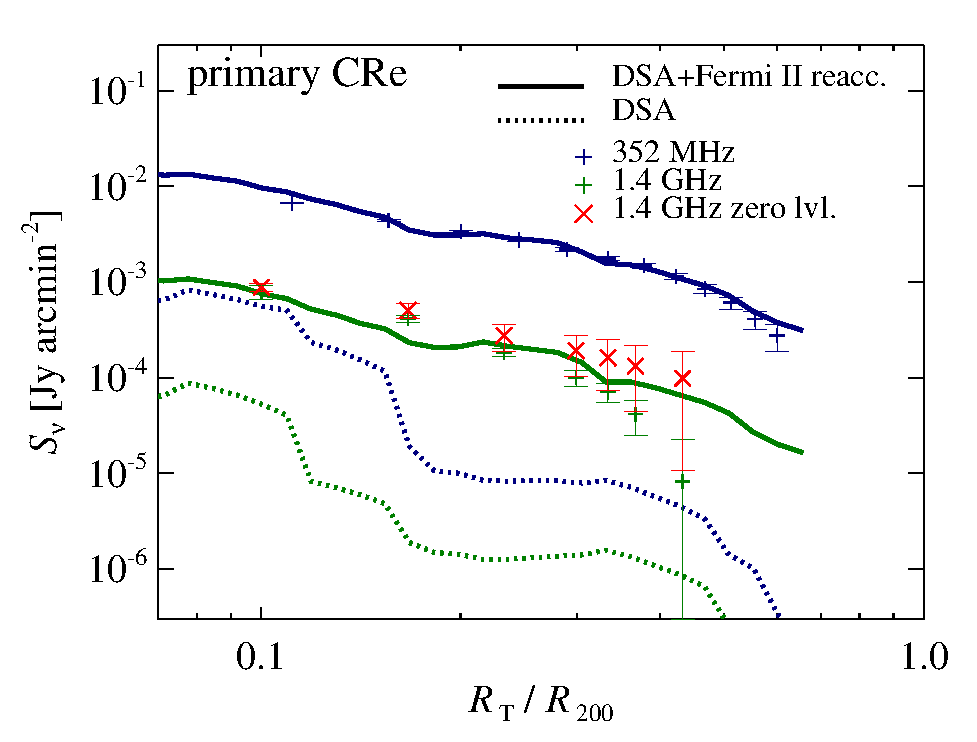
\includegraphics[width=\columnwidth]{sbright.nu.DIIcomp.Pri.g72a.Rad14.2400p.z0.NL.xKR.eb23.eI088.140.v6.eps}
   \end{center}
\end{minipage}
\begin{minipage}{1\columnwidth}
   \begin{center}\Large{\Mstream:}\\
     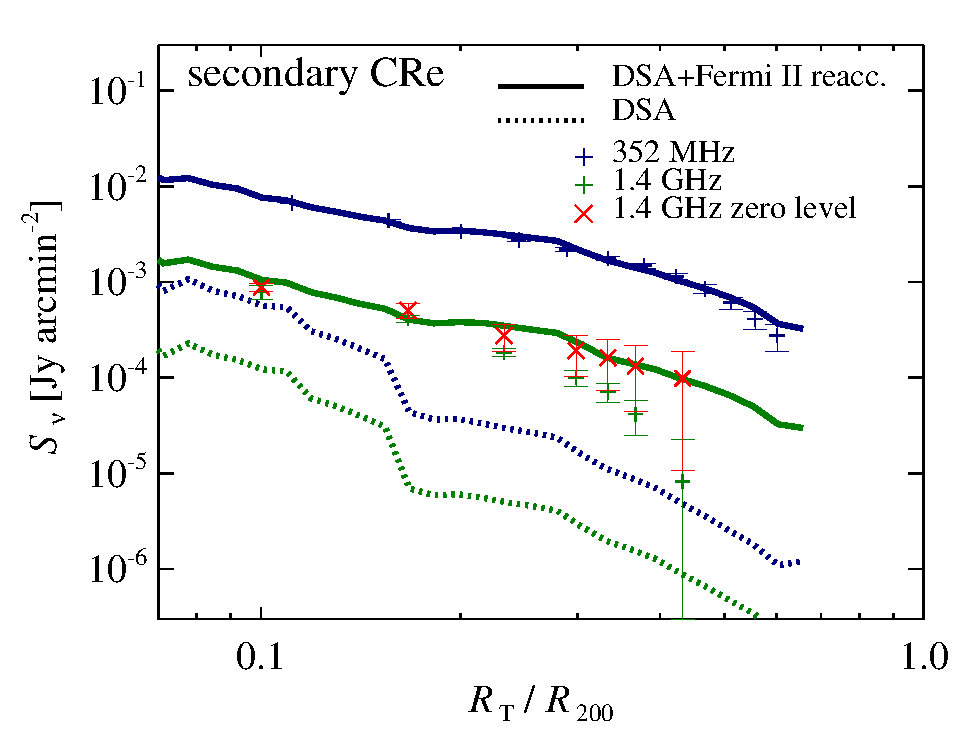
\includegraphics[width=\columnwidth]{sbright.nu.DIIcomp.flatCR.g72a.Rad14.2400p.z0.NL.xKR.eb23.eI082.flatCR.140.v6.eps}
   \end{center}
\end{minipage}
\\
\begin{minipage}{1\columnwidth}
  \begin{center}\Large{\Mflatturb:}\\ 
    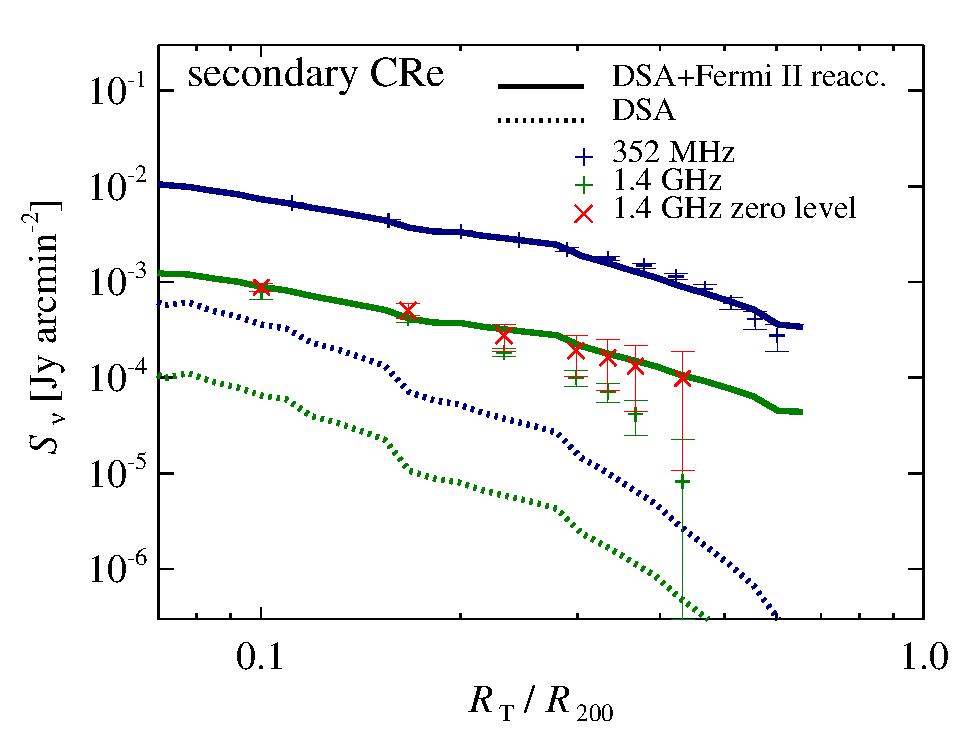
\includegraphics[width=\columnwidth]{sbright.nu.DIIcomp.I0.g72a.Rad14.2400p.z0.NL.xKR.eb23.eI067.140.v6.eps}
  \end{center}
\end{minipage}
\begin{minipage}{1\columnwidth}
   \begin{center}\Large{\it Brunetti et al. (2012)}:\\
     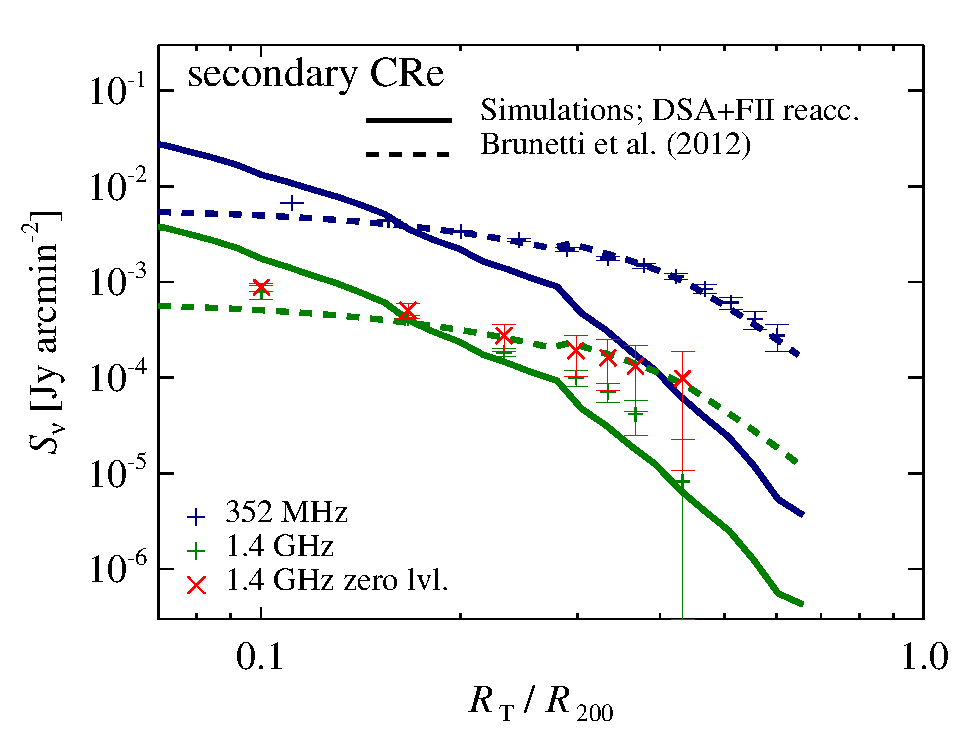
\includegraphics[width=\columnwidth]{sbright.nu.DIIcomp.Brunetti.g72a.Rad14.2400p.z0.NL.xKR.eb23.140.v6.eps}
   \end{center}
\end{minipage}
\caption{Radio surface brightness profiles of Fermi-II reaccelerated
  CR electrons of a simulated post-merging cluster similar to Coma. We
  compare profiles at 352~MHz \citep[blue lines and
    crosses,][]{brown11} to those at 1.4~GHz \citep[green lines and
    crosses,][]{deiss97}. The red crosses show the reprocessed 1.4~GHz
  data, where a zero level of about 10~\% of the central value is
  adopted. The solid lines show predicted emission from a
  reaccelerated fossil population, while dotted lines show emission
  from a fossil population without reacceleration. The panels show the
  emission of our models \Mprimary (upper left panel), \Mstream (upper
  right panel), \Mflatturb (lower left panel), and simulated secondary
  electrons together with previous estimates \citep{brunetti12} for
  the Coma cluster (lower right panel).}
  \label{fig:sync_profile}
\end{figure*}

In Fig.~\ref{fig:sync_profile}, we show radial profiles for the radio
emission in all three scenarios in which the seeds undergo Fermi-II
reacceleration in turbulent fields that are shaped such as to
reproduce the Coma RH profile at 352~MHz.  Adopting our
parametrisation for the volumetric injection rate of turbulent energy,
$I_0\propto \eps_\rmn{th}^{\alpha_\rmn{tu}}$, we find that to fit the observations, we require
$\alpha_\rmn{tu}= 0.67$ for \Mflatturb, $\alpha_\rmn{tu}= 0.82$ for
\Mstream, and $\alpha_\rmn{tu}= 0.88$ for \Mprimary. As a result, the
ratio of turbulent-to-thermal energy densities slightly increase with
radius as shown in Fig.~\ref{fig:turb}.  The fine-tuning of these exponents is somewhat problematic, as we discuss in \S\ref{sect:param_comp}. After turbulent
reacceleration, the volume-weighted, relative CRp energy density and
relative CRp number density inside the RH for \Mflatturb (\Mstream),
are found to be 2 (3) \% and $2\times10^{-8}$ ($5\times10^{-8}$),
respectively.


\begin{figure}
  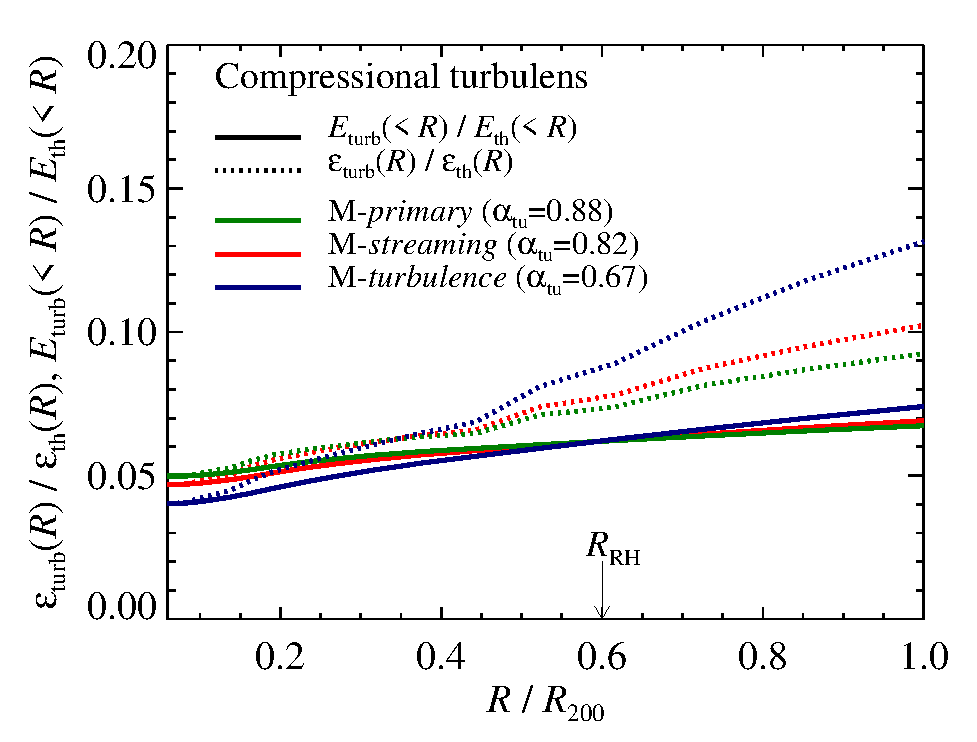
\includegraphics[width=1.0\columnwidth]{turb_profile_ratio_tot.eps}
  \caption{The ratio of turbulent-to-thermal energy densities (solid
    lines) and cumulative energies (dotted lines) in our three
    models. The energy densities are parametrized as
    $\eps_\rmn{turb} \propto
    \eps_\rmn{th}^{(\alpha_{\rmn{tu}}+1)/2}/T^{1/4}$ and
    normalized such that the total turbulent energy in compressible
    modes $E_\rmn{turb}$ for each scenario makes up about 20\% of the
    total thermal energy $E_\rmn{th}$ inside the radio halo
    ($R_\rmn{RH}\approx0.6R_{200}$). The turbulent profiles explore
    the uncertainty in the cluster turbulence and are motivated by the
    cosmological simulation in
    \citep{2009ApJ...705.1129L,2010ApJ...725.1452S,2011A&A...529A..17V}.}
  \label{fig:turb}
\end{figure}

Figure~\ref{fig:sync_profile} demonstrates that the modeled radio
profiles without turbulent reacceleration are too steep.  In the
bottom right panel of Fig.~\ref{fig:sync_profile} (labeled with
Brunetti et al. 2012), we show that our simulated profiles of
reaccelerated CRs, which only take advective CR transport into
account, i.e. they neglect CR streaming or a flatter turbulent
profile, produce radio profiles that are too steep. Indeed, even using
the assumptions of previous work -- where complete freedom in the seed
population was allowed -- it is not possible to reproduce observations
in both frequencies in any model.\footnote{Note that in previous work
  on the Coma cluster, $\eps_\rmn{turb} \propto \eps_\rmn{th}$ was
  adopted which approximately corresponds to $\alpha_\rmn{tu}= 1$
  \citep{brunetti12} and together with the different distributions for
  seed CRes constitute the main differences compared to our work.}
Decreasing the acceleration efficiency with radius does not change
this conclusion much because of the weak radial dependence of
$D_{\rm pp}(R)\propto \eps_\rmn{th}(R)^{\alpha_\rmn{tu}-1}
\sqrt{T(R)}$. This signals that the problem is generic and requires
either additional modifications to the plasma physics of acceleration
or a better understanding of potential observational systematics. In
addition there are differences in the simulated density and
temperature profiles in comparison to the observed profile in Coma
that impact the CR abundance as well as cooling and reacceleration.

In Figure~\ref{fig:tauD} we show how the turbulent reacceleration
timescales in our three models scale with radius. As expected, the
\Mprimary model with $\alpha_\rmn{tu}=0.88$ has the flattest profile
with $\tau_{\rm D}\approx0.4\,\rmn{Gyr}$, where the small dip at large
radius driven by the decrease in thermal energy density. The
\Mflatturb model has the the flattest turbulent profile parameterized
by the smaller $\alpha_\rmn{tu}$ which explains the steepest $\tau_{\rm D}$
profile. Note that a fixed reacceleration timescale is required to
explain the observations at each radius and for each model (see also
Table~\ref{tab:timescales}). Since $\tau_\rmn{cl} \propto X_\rmn{tu}^2 k_0$,
these two parameters are degenerate and can be traded off one another.

\begin{figure}
  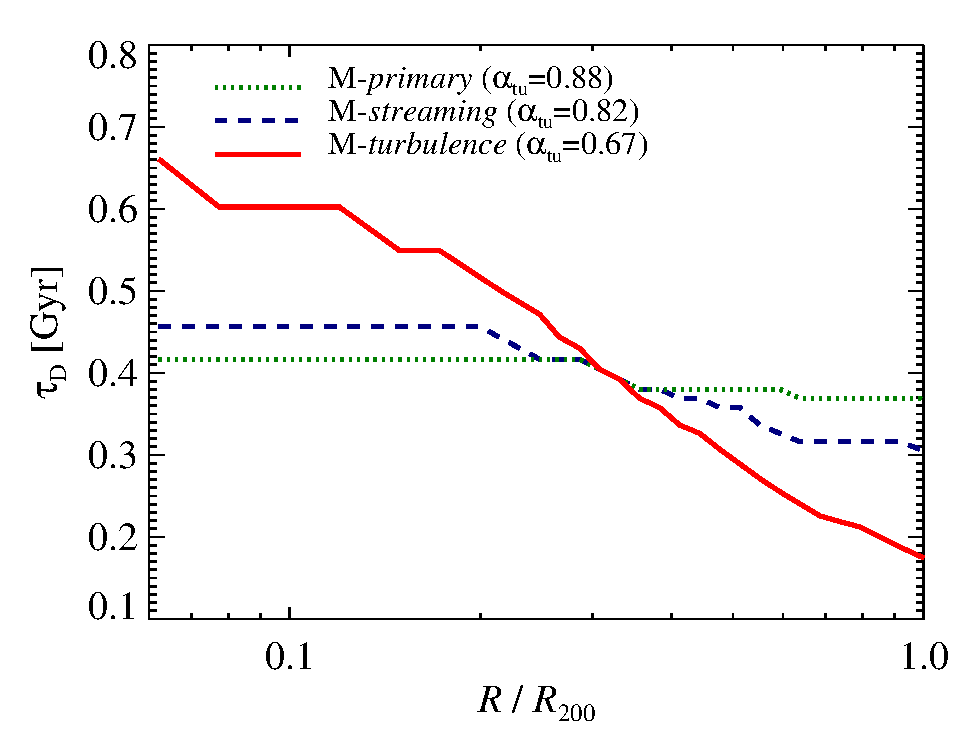
\includegraphics[width=1.0\columnwidth]{tau_reacc.eps}
  \caption{Turbulent reacceleration timescales for our simulated
    cluster g72a. We show in linear-log the reacceleration timescale
    ($\tau_{\rm D}$) as a function of radius $R$ for our three models:
    \Mprimary (green dotted line), \Mstream (blue dashed line), and
    \Mflatturb (red solid line). Note that the timescales are derived
    during the last 100~Myrs in time in our simulations.}
  \label{fig:tauD}
\end{figure}

In principle, reacceleration via TTD leads to spectral steepening with
particle energy due to the inefficiency of the acceleration process to
counter the stronger cooling losses with increasing energy. Since
synchrotron emission peaks at frequency $\nu_\rmn{syn}\simeq 1\,
B/\umu\rmn{G} (\gamma/10^4)^2\,\rmn{GHz}$, this translates into a
spectral steepening of the radio spectrum (see the left panel of
Fig.~\ref{fig:sync_spectrum} where the continuous injection of
secondary CRes is absent). A given radio window samples higher energy
electrons for a decreasing field strength in the cluster
outskirts. Hence, the spectral steepening with energy should translate
into a radial spectral steepening \citep{brunetti12}. However, because
of the weak dependence of the electron Lorentz factor on emission
frequency ($\gamma\propto\sqrt{\nu_\rmn{syn}}$), this effect is only
visible in our simulations for $\nu_\rmn{syn}\gtrsim5$~GHz. Most
importantly, our simulated fluid elements at a given radius sample a
broad distribution of shock history, density and temperature, which
implies very similar synchrotron brightness profiles at
$\nu_\rmn{syn}=352$~MHz and 1.4 GHz. The discrepancy of the observed
and simulated 1.4 GHz profiles could instead be due to systematic flux
calibration error in single dish observations. These could arise, for
instance, due to errors in point source subtraction. Interestingly, we
can match the 1.4 GHz data if we reduce the zero point by adding 10\%
of the central flux to every data point; this flattens the outer
profile\footnote{Lawrence Rudnick, private communication.}.
Alternatively, this may point to weaknesses in the theoretical
modeling of the particle acceleration process and may require a
stronger cutoff in the particle energy spectrum.


\subsection{Radio spectrum}
\label{sect:radio_spec}
In Fig.~\ref{fig:sync_spectrum} we show that our three models that
include Fermi-II reacceleration can individually reproduce the
convexly curved total radio spectrum found in the Coma cluster. Seed
CRs in \Mstream and \Mflatturb that do not experience turbulent
reacceleration have a power-law spectrum in disagreement with
observations. In order to match both the spatial and spectral profiles
in Coma, we adopt an acceleration efficiency for the strongest shocks
in our three models \Mprimary, \Mstream, and \Mflatturb to
$\zeta_{\rmn{e}} <0.003$, $\zeta_{\rmn{p}} < 0.1$, and
$\zeta_{\rmn{p}}<0.03$, respectively. Following the Mach number
($\mathcal{M}$)-dependence of the acceleration efficiency suggested in
\cite{pinzke13}, the efficiency in weak shocks ($\mathcal{M}\sim
2.5-3.5$) that dominates the CR distribution function, has an
acceleration efficiency for protons $\zeta_{\rmn{p}}\sim0.0001-0.01$,
and for electrons $\zeta_{\rmn{e}}\sim 0.001$.

Interestingly, we find that the radio luminosity from clusters in the
OFF-state (DSA only) and ON-state (DSA and reacceleration) differ by
about a factor 10-20 in all our three models. This means that the
secondary CRes are dominated by the reaccelerated fossil CRes and not
from the CRes produced by reaccelerated CRps. However, for high
frequencies ($\nu_\rmn{syn}\gtrsim$ GHz) where synchrotron cooling is
more efficient than reacceleration, the emission is dominated by the
CRes produced in the continuous injection of electrons from
reaccelerated CRps. It is also worth mentioning that the radio
emission from secondary CRes are smoothly distributed around the
cluster because of the continuous injection, hence the it is not
dominated by outliers.

However, for \Mprimary, the primary CRes that generate most of the
radio emission from the cluster in the OFF-state are dominated by only
a small fraction of the CRes. These electrons are injected very
recently and have not had time to cool yet. Hence we expect there to
be a large variance in the OFF-state of different simulated
clusters. As mentioned in section~\ref{sect:param_comp}, combining
radio observations with gamma-ray limits allows us to put a lower
limit to $X_\rmn{tu}$.  If $X_\rmn{tu}$ is smaller than in our adopted
models (where we assume $X_\rmn{tu}=0.2$), then the efficiency of DSA
has to be larger than $\zeta_\rmn{p}\sim 0.1$ for the secondary CRes
to reproduce the radio observations. However, since the turbulent
reacceleration acts on both the secondary CRes and the CRps, while
$\zeta_\rmn{p}$ only affects the CRps, \Mstream and \Mflatturb would
produce too much gamma-rays. Hence we conclude that
$X_\rmn{tu}\gtrsim0.2$ if all other parameters are kept
fixed. Although, we caution the reader to take this limit too
stringent because of the uncertainty in $k_0$ and $\tau_\rmn{cl}$ that
impact $X_\rmn{tu}$ for a fixed $\tau_\rmn{D}$. This parameter space
needs to be explored further in future work in order to put more
stringent limits on the level of turbulence in clusters using radio
and gamma-ray observations in combination with turbulent reaccelerated
CRs.

\begin{figure*}
  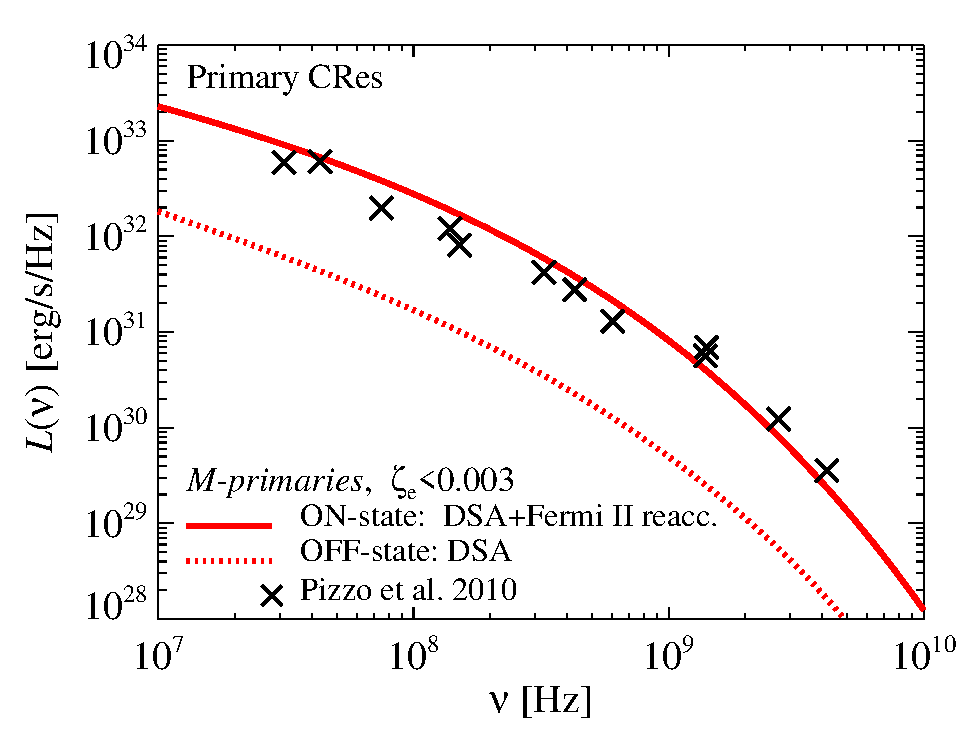
\includegraphics[width=1.0\columnwidth]{sync.spec.pri.g72a.140.v6.eps}
  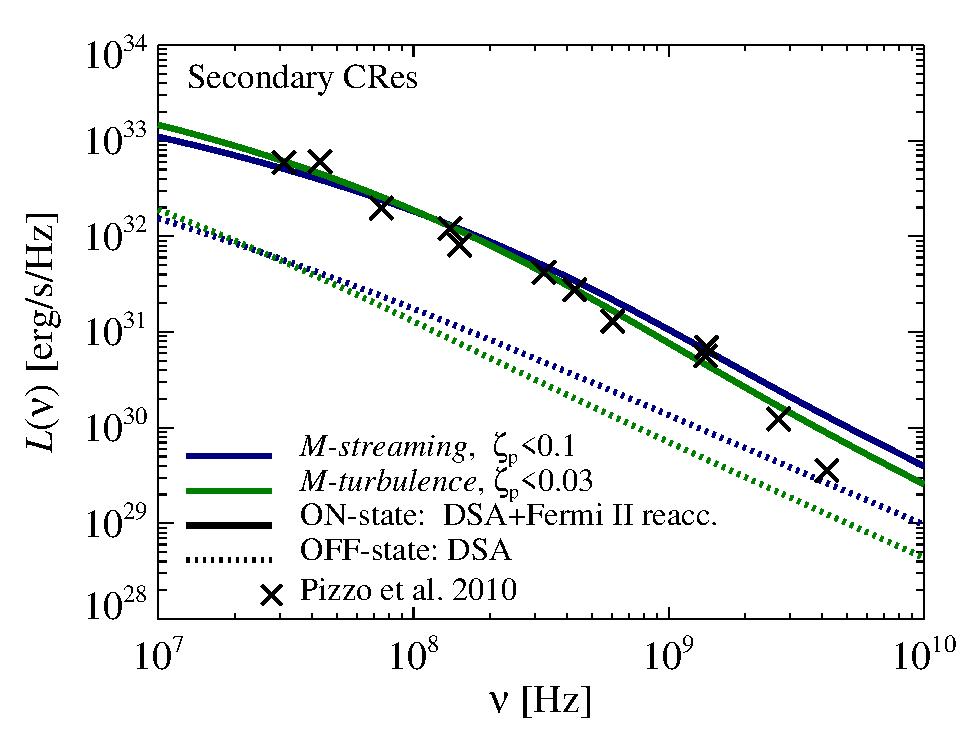
\includegraphics[width=1.0\columnwidth]{sync.spec.sec.g72a.140.v6.eps}
  \caption{Radio synchrotron spectra. Lines are derived from
    simulations, while the black crosses are compiled from
    observations \citet{2010PhDT.......259P}. The solid lines show the
    DSA and reaccelerated CRs (On-state of the radio halo), while the
    dotted lines show CRs accelerated only by DSA (Off-state of the
    radio halo). The left figure shows the radio emission induced by
    primary CRes and the right figure shows the emission from
    secondary CRes. The different line colors represent our different
    models, \Mprimary (red line), \Mstream (blue line), and \Mflatturb
    (green line).}
  \label{fig:sync_spectrum}
\end{figure*}

\subsection{Gamma rays}
The gamma-ray emission from CRps that produce decaying neutral pions
could be substantial if the CRps are reaccelerated efficiently enough,
hence it is interesting to estimate this emission for our models and
compare to upper limits. We follow the formalism outlined in
  \cite{1999APh....12..169B} (and references therein) and calculate
  the gamma-ray emission numerically for our three models. We predict
the gamma-ray emission from \Mflatturb (\Mstream) with
$F_\gamma(>500\,\rmn{MeV})=4\times10^{-10} (5\times10^{-10}) \mathrm{
  \,ph\, s}^{-1}\mathrm{cm}^{-2}$. The fluxes from these models are
slightly larger than in \cite{brunetti12}, where the differences comes
from our steeper CRp profiles in addition to simulation based
formalism we rely on that accounts for both Coulomb and hadronic
losses during the build up of the CR distribution in contrast to the
scaling relations adopted in their paper. Interestingly the gamma-ray
flux from both our scenarios are just below recent Fermi-LAT limits
derived from a gamma-ray profile similar to \Mflatturb where
$F_\gamma(>500\,\rmn{MeV})<5.3\times10^{-10} \mathrm{ \,ph\,
  s}^{-1}\mathrm{cm}^{-2}$ \footnote{Fabio Zandanel, private
  communication. See also
  \citet{2014MNRAS.440..663Z,2014ApJ...787...18A}. and will be probed
  in the next few years by Fermi-LAT. } The spectral index of the CRp
distribution is relatively steep ($\alpha_{\rmn{p}}\sim2.6$) for the
CRp energies $E \gtrsim 10$~GeV that are relevant for the injection of
radio-emitting secondary CRes. The steep spectrum is ultimately a
consequence of the shock history of the simulated cluster, with a weak
dependence on our test particle model for Fermi-I acceleration
\citep{pinzke13}, where we steepen the spectral index to avoid
acceleration efficiencies above $\zeta_{\rmn{p}} \sim 10\%$.


% --- section: Analytical Results and discussion --- %
\section{Parameter Space Exploration and Overcoming Fine Tuning}
\label{sect:param_comp}
In this paper we rely on several critical parameters describing
relatively unknown non-thermal physics in the ICM. Here we develop a
simplified framework for our reacceleration model of secondary
electrons. We will explore how radio emission depends on the
parameters describing the spatial profile of CR protons and
turbulence. Our fiducial model is meant to be
compared against the Coma cluster.


\subsection{Methodology}

As we have seen before, the most uncertain aspects of radio halo
emission models are the profile of compressible turbulence (which
determines the amount of Fermi II acceleration) and the distribution
of pre-existing CRs. Hence we vary parameters describing the amount of
energy contained in turbulence, $X_{\rm tu}$ (defined by $E_{\rm
  turb} = X_{\rm tu} E_{\rm th}$), the spatial profile of
turbulence as parametrized by $\alpha_{\rm tu}$ (defined by $I_0
\propto \eps_{\rm th}^{\alpha_{\rm tu}}$, where $I_0^{} \propto
\varv_0^{3} k_0^{}$ is the injection rate of turbulence), as well as
the spatial CR profile that we will parametrize by $\alpha_{\rm CR,
  spat}$ (see below).  We hold fixed thermal plasma properties
(temperature and density profiles), $B$-field profiles, total CR energy
content, and the turbulent outer scale (corresponding to a wavenumber
$k_{0}$). The CR energy content is suggested by our simulations
(observations only give an upper bound;
\citealt{2012ApJ...757..123A}). We focus on the uncertain CR
distribution rather than the overall normalization, since the impact
of the latter (an overall linear scaling) is clear.

In order to quickly explore this parameter space, we solve the
Fokker-Planck equation in static spherical shells for injection,
reacceleration, and losses of the CRs, i.e., we neglect Lagrangian
evolution during re-acceleration.  This ignores the effect of
adiabatic compressive heating of the CRs, though this is generally
subdominant (e.g., see Fig. 7 of \citealt{miniati15}). Once
the CRs have been reaccelerated for $\tau_\rmn{cl} = 650\,\rmn{Myr}$,
we calculate the resulting radio emission numerically using the
formalism outlined in \cite{1979rpa..book.....R} and compare the
emission profiles and spectra as we vary one parameter at a time
relative to our fiducial model.

We adopt both the density \citep{1992A&A...259L..31B} and temperature
profiles \citep{2009ApJ...696.1886B,2001A&A...365L..67A} derived from
X-ray observations of the Coma cluster,
\begin{eqnarray}
n_e &=& n_0\,\left[1+\left(R/R_{\rmn{c}}\right)^2\right]^{-1.125},\nonumber\\
k_{\rmn{B}} T &=& 8.25\,\rmn{keV} \left[1+\left(2R/R_{200}\right)^2\right]^{-0.32},
\end{eqnarray}
with $n_0=3.4\times10^{-3}\,\rmn{cm}^{-3}$.  The virial and core radii
of Coma are given by $R_{200} = 2.3\,\rmn{Mpc}$
\citep{2002ApJ...567..716R} and $R_{\rmn{c}} = 294\,\rmn{kpc}$,
respectively. In accordance with Faraday rotation measure
measurements, we assume $B(r)=B_{0} (n/n_{0})^{\eta}$, where
$B_{0}=4.8 \mu$G and $\eta=0.5$ \citep{bonafede10}.

The bulk of the CRps are injected by relatively low Mach number shocks
and parameterized by $f_\rmn{p,inj}(p) =
C_\rmn{inj}\,p^{-\alpha_\rmn{inj}}$, where $\alpha_\rmn{inj}\approx
2.5$ in our simulations. The CRps approximately trace the thermal gas
with $C_\rmn{inj} \propto \eps_\rmn{th}^{\alpha_\rmn{CR,spat}}$
\citep{pinzke10,2016MNRAS.459...70V}, where the normalization is fixed
by the injected CR energy in the last 650~Myrs. Our simulations show
that it approximately amounts to 0.03\% of the thermal energy inside
the virial radius, i.e.  $\int_0^{R_{200}}\eps_\rmn{p,inj} \rmn{d}
V\left(\int_0^{R_{200}}\eps_\rmn{th} \rmn{d}V\right)^{-1} =
0.0003$. The spectrum of the initial CRp distribution is determined by
the steady state between injection and cooling,
\begin{equation}
 f_\rmn{p,0} \propto \frac{\int_p^\infty f_\rmn{p,inj}(p') 
\rmn{d}p'}{\displaystyle\left|{{\rmn{d}p}\over{\rmn{d}t}}\right|_{\rm Coul}+\frac{p}{\tau_{\rm had}}}\,,
\end{equation}
where we fix the normalization by requiring
$\int_0^{R_{200}}\eps_\rmn{p,0}
\rmn{d}V\left(\int_0^{R_{200}}\eps_\rmn{th} \rmn{d}V\right)^{-1} =
0.003$. Note that the injected energy in the last 650 Myr is smaller
by about a factor of 10 in comparison to the cumulative CR energy
injected over the entire cosmological history of the cluster, but this component is nonetheless important since above 1 GHz the radio emission is dominated by CRe's injected during the merger, which have not yet had time to cool. 
Similarly, the initial CRe distribution is given by the steady state
between cooling (Coulomb, inverse Compton, and synchrotron) and
injection of secondary CRes from $f_\rmn{p,0}$. 
The diffusion constant $D_{\rm pp} \propto X_{\rm tu}^{2}
\eps_{\rm th}^{\alpha-1} \sqrt{T} k_{\rm 0}$ is calculated for each
radial bin. All parameters
and assumptions are similar to what is used for our simulated cluster
(see Sect.~\ref{sec:results}). Our fiducial model assumes $X_{\rm tu}
= 0.2$, $\alpha_{\rm tu} =0.8$, $\alpha_{\rm CR, spat}=1.0$, and
$k_{\rm 0}=2 \pi/\lambda_{\rm 0}$ where $\lambda_{\rm 0}=100$ kpc. We
also assume a fixed acceleration time of $\tau_{\rm cl} = 650 \, {\rm
  Myr}$.


\subsection{Results}

\begin{figure*}
\begin{minipage}{1\columnwidth}
   \begin{center}\Large{radio profiles}\\
     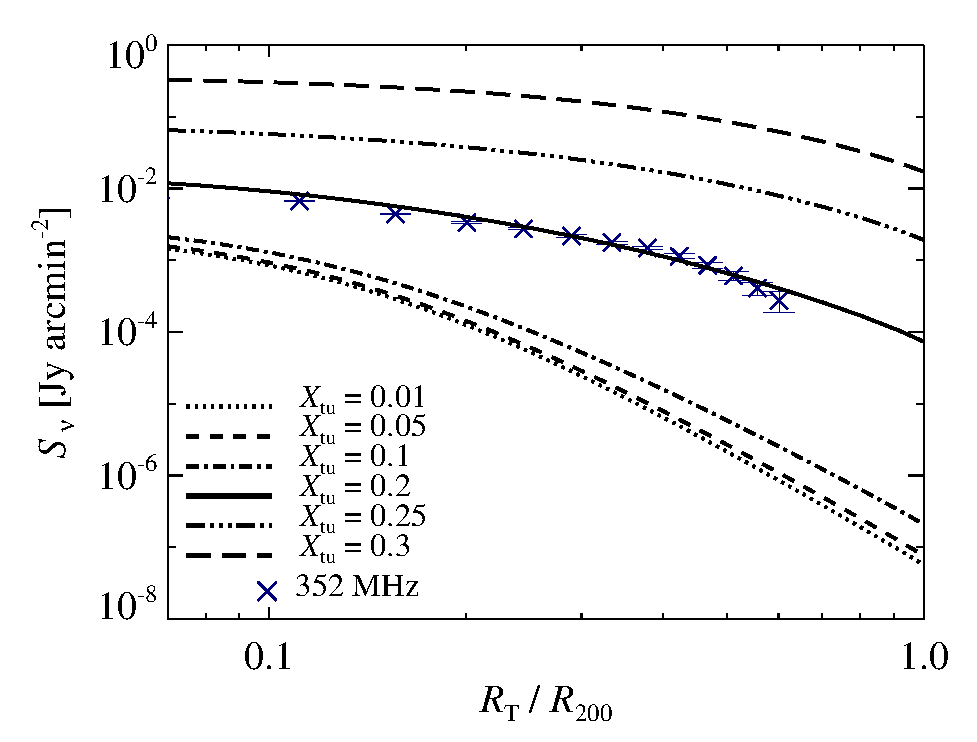
\includegraphics[width=\columnwidth]{prof.comp.KrTTDth.Xtu.eps}
   \end{center}
\end{minipage}
\begin{minipage}{1\columnwidth}
   \begin{center}\Large{radio spectra}\\
     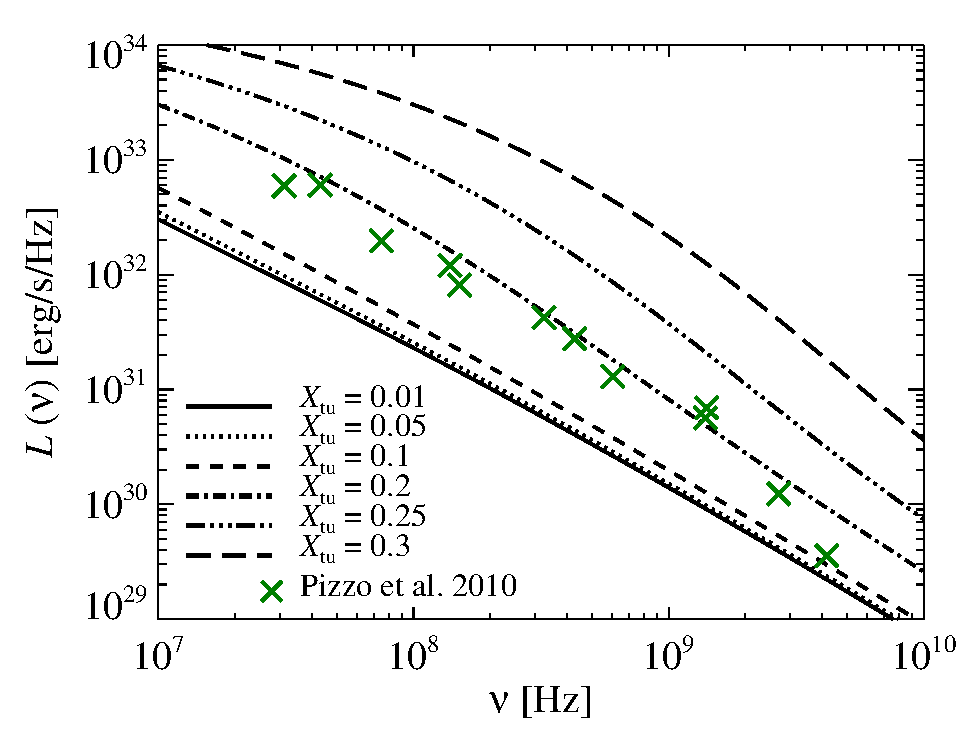
\includegraphics[width=\columnwidth]{spec.comp.KrTTDth.Xtu.eps}
   \end{center}
\end{minipage}
\\
\begin{minipage}{1\columnwidth}
  \begin{center}%\Large{\Mflatturb:}\\ 
    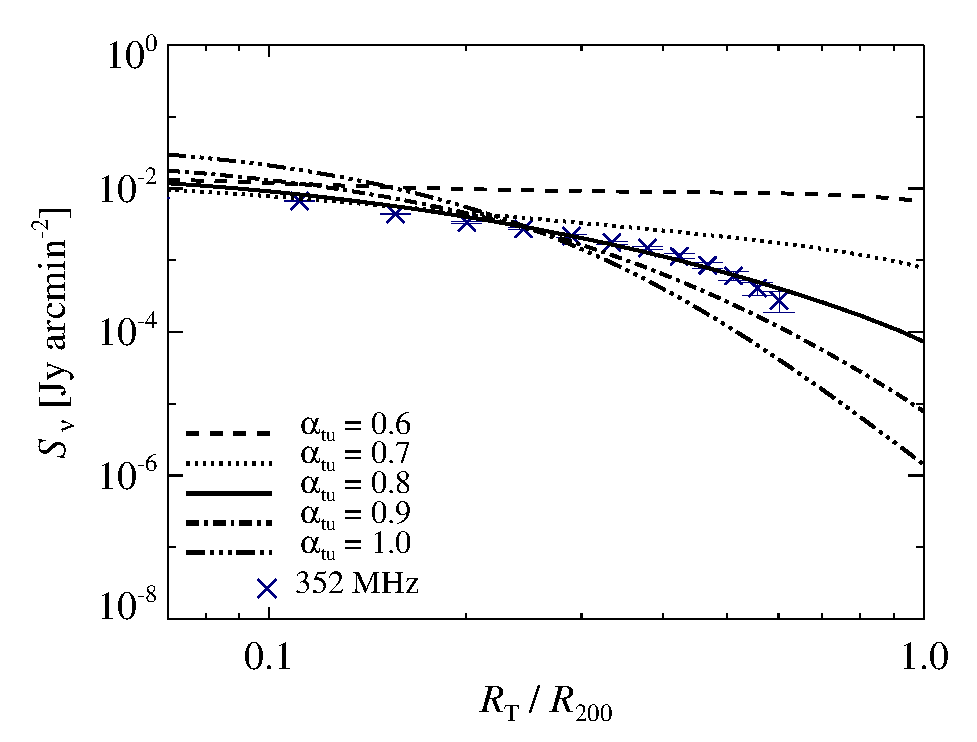
\includegraphics[width=\columnwidth]{prof.comp.KrTTDth.aI0.eps}
  \end{center}
\end{minipage}
\begin{minipage}{1\columnwidth}
   \begin{center}%\Large{\it Brunetti et al. (2012)}:\\
     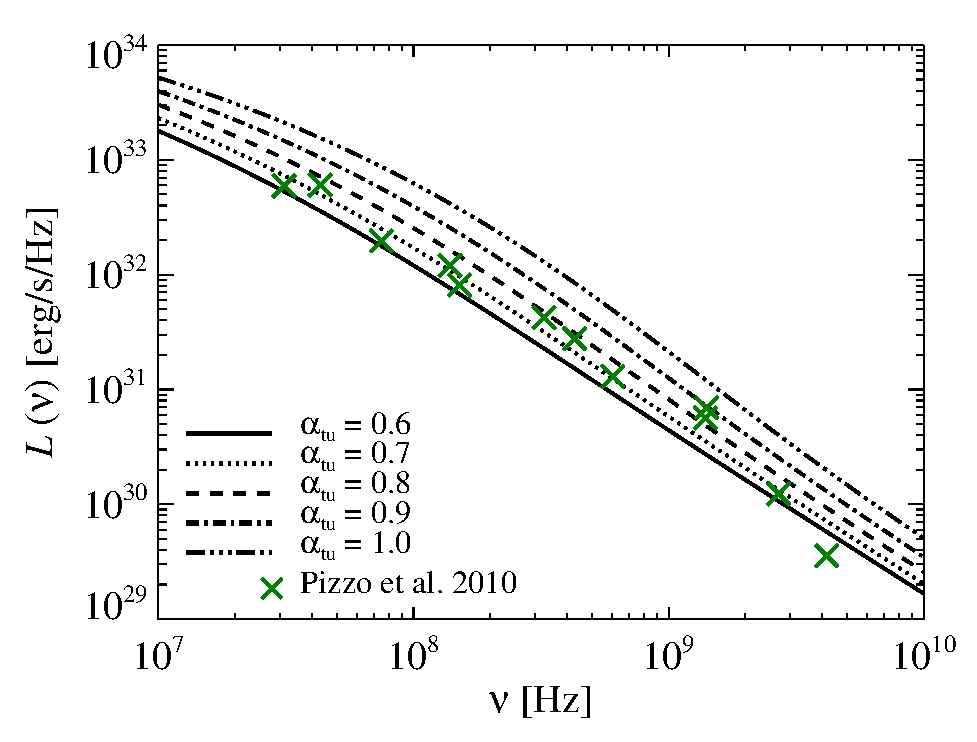
\includegraphics[width=\columnwidth]{spec.comp.KrTTDth.aI0.eps}
   \end{center}
\end{minipage}
\\
\begin{minipage}{1\columnwidth}
  \begin{center}%\Large{\Mflatturb:}\\ 
    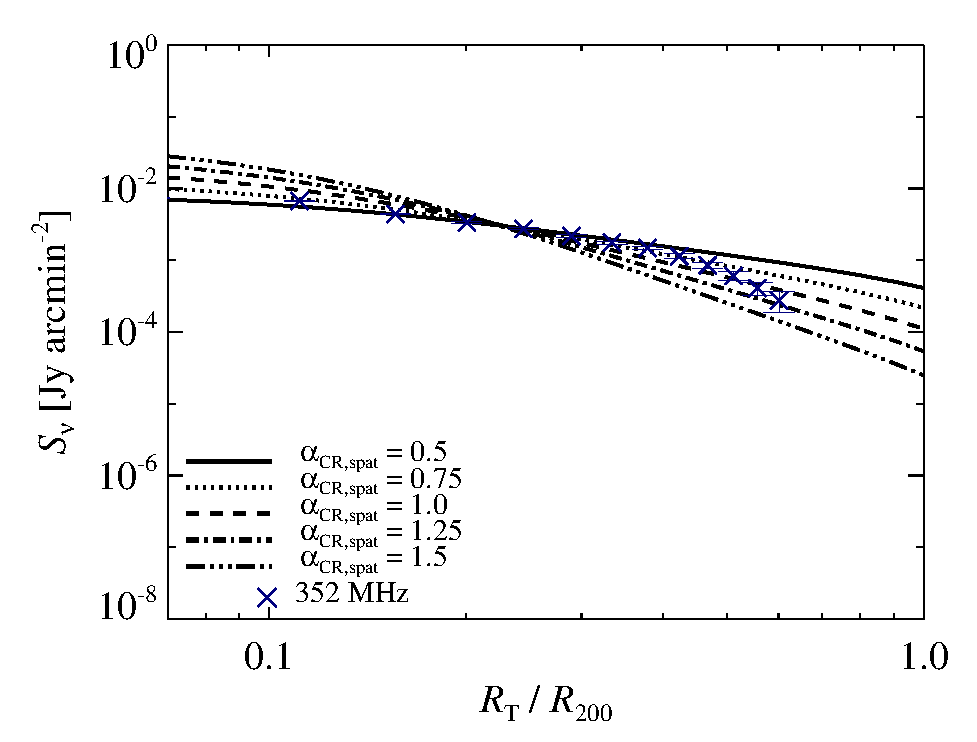
\includegraphics[width=\columnwidth]{prof.comp.KrTTDth.aCR.eps}
  \end{center}
\end{minipage}
\begin{minipage}{1\columnwidth}
   \begin{center}%\Large{\it Brunetti et al. (2012)}:\\
     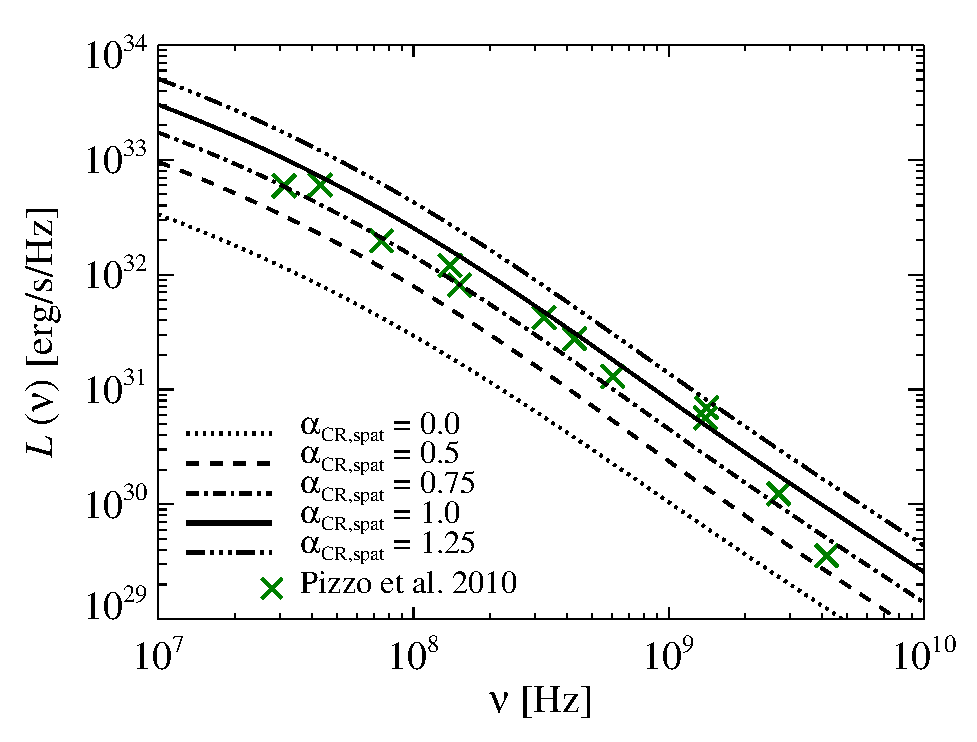
\includegraphics[width=\columnwidth]{spec.comp.KrTTDth.aCR.eps}
   \end{center}
\end{minipage}
\caption{Sensitivity of radio emission in Coma cluster to critical
  parameters. The left-hand panels show the radio surface brightness
  profiles. We compare profiles at 352~MHz \citep[blue
    crosses,][]{brown11} to predicted emission from Fermi-II
  reaccelerated CR electrons populations (black lines). The right-hand
  panels show radio synchrotron spectra. The green crosses are
  compiled from observations \citep{2010PhDT.......259P}, while the
  black lines show predicted spectra. The upper panels show the sensitivity to the level of
  turbulence ($X_\rmn{tu}$), the middle panels show the impact of
  different turbulent profiles ($\alpha_\rmn{tu}$), and the lower
  panels show the dependence on spatial distributions of initial and
  injected CRs ($\alpha_\rmn{CR,spat}$). We adopt the following
  fiducial values for our model, $X_\rmn{tu}=0.2$,
  $\alpha_\rmn{tu}=0.8$, and $\alpha_\rmn{CR,spat}=1.0$ and vary each
  parameter separately in each row of panels. We find that the radio
  emission is most sensitive to the level of turbulence. The abundance of CR seeds, and the spatial distribution of CRs and turbulence play second-order effects.}
  \label{fig:param_comp}
\end{figure*}

Figure~\ref{fig:param_comp} shows the impact of turbulence and the
spatial distribution of CRs on the radio emission. 

{\bf Impact of overall level of turbulence ($X_{\rm tu}$).} From the top panels of Fig.~\ref{fig:param_comp}, we see that as $X_{\rm tu}$ increases, there are 3 important changes: an exponential increase in radio luminosity, a flattening of the radio surface brightness profile, and an increase in spectral curvature. We discuss these in turn. 

As we show in \S\ref{sect:self-limiting}, the exponential increase in radio surface brightness is easily understood from equation~\ref{eq:Creacc}, since for a power-law initial distribution function $f_{\rm i}(p) = C_{\rm 0} p^{-\alpha}$, then $C_{\rm reacc} \propto C_{\rm 0} {\rm exp}(A \tau_{\rm cl}/\tau_{\rm D}) \propto {\rm exp} (B(r) X_{\rm tu}^{2})$. This exponential sensitivity is somewhat modified by cooling (which results in a non power-law spectrum; also, the shorter the acceleration time, the larger the pool of seed electrons available which would otherwise cool away), but overall is a good approximation.  

An increase in $X_{\rm tu}$ flattens the surface brightness profile, since high acceleration efficiency leads to larger amplification in the cluster outskirts (where cooling is less important) than the center. In particular, in the cluster outskirts, the reduced impact of Coulomb cooling implies that there is a larger pool of low-energy electrons available for reacceleration (see timescales in Table \ref{tab:timescales}). 

Larger levels of turbulence also {\it increase} spectral curvature, which might seem puzzling. It can be understood as follows. The pre-acceleration electron distribution function results from the competition between hadronic injection $f \propto p^{-\alpha_{\rm inj}}$ and cooling, which results in a quasi-steady state for the non-thermal (secondary) electrons. At low momenta, when the Coulomb cooling time is short, $f \propto p^{-\alpha_{\rm inj}+1}$, at high momenta, when inverse Compton/synchrotron cooling dominates, $f \propto p^{-\alpha_{\rm inj} -1}$. In between, there is a quasi-adiabatic regime where electrons accumulate (for more details, and an analytic self-similar solution, see \citealt{1999ApJ...520..529S, pinzke13}). In the absence of cooling, momentum advection in the limit $D_{\rm pp} \propto p^{2}$ (so that $\tau_\rmn{D} =p^{2}/4 D_{\rm pp}$ is momentum independent) simply shifts the distribution $f(p) \rightarrow f(A p)$. 
When the acceleration efficiency is low, most observable emission corresponds to the power-law tail of the distribution function $f \propto p^{-\alpha_{\rm inj}-1}$ set by the balance between injection and synchrotron/IC cooling. However, as the acceleration efficiency $A$ increases, radio emission starts to probe the 'bump' around $p_{*}$ (given by $\tau_{\rm D} \sim \tau_{\rm cool}(p_{*})$) where electrons accumulate and the distribution function is curved. This results in a curved emission spectrum. The synchrotron spectrum steepens at the frequency \citep{2001MNRAS.320..365B}: 
\begin{equation}
\nu_{\rm s} \propto \frac{B \tau_{\rm D}^{-2}}{(B^{2}+B^{2}_{\rm CMB})^{2}}
\end{equation}
where $B_{\rm CMB} \equiv (8 \pi U_{\rm CMB})^{1/2}$, which increases for shorter $\tau_{\rm D}$.  

{\bf Impact of spatial profile of turbulence ($\alpha_{\rm tu}$).} From the middle panels of Fig.~\ref{fig:param_comp}, we see that as expected, a flatter profile of the turbulent pressure directly translates into a flatter radio surface brightness profile. Since seed electrons are more concentrated toward the center (the collisional production of secondaries is more rapid there), and magnetic fields are stronger, concentrating the turbulence toward the cluster center for fixed $X_{\rm tu}$ results in higher radio luminosities, and slightly more curvature (due to the increased importance of cooling near the center). Overall, however, the spatial profile of turbulence has a much weaker effect than its overall normalization. 

{\bf Impact of spatial profile of seed CRs $\alpha_{\rm CR, spat}$.} The spatial distribution of CRs has an even smaller impact on radio emission. At fixed total CR energy content $X_{\rm CR}$, concentrating the CRs towards the center leads to more centrally dominated surface brightness profiles, as expected, and higher radio luminosities (for the same reasons as above: secondaries are more easily produced in the center, and magnetic fields are stronger). We have also confirmed that radio surface brightness profiles scale linearly with $X_{\rm CR}$, as expected. 

Overall, our results suggest that radio halos are much more sensitive to the level of turbulence (exponential dependence) rather than CR abundance (linear dependence), and that the spatial distribution of turbulence and CRs, while important, are second-order effects. In our parametrization, the most important controlling variable is $X_{\rm tu}$. The overall level of turbulence has to be such that $\tau_{\rm D} \sim \tau_{\rm cl}$ (see Table \ref{tab:timescales}), otherwise, too little or too much amplification takes place. For instance, for $X_\rmn{tu}\gtrsim0.08$, changing $X_\rmn{tu}$ by a factor of two changes the radio surface brightness by a factor of $\sim 10-100$ (see top panels of Fig.~\ref{fig:param_comp}). The required $\tau_{\rm D}/\tau_{\rm cl}$ depends only logarithmically on the abundance of seed CRs.

While the requirement of a threshold level of turbulence may explain why radio brightness is bimodal, it also raises a fine-tuning problem: why is the $L_{\rm radio}$ vs. $L_{\rm X}$ relation in active radio halos so tight? Depending on the details of infall or mergers, we would naturally expect fluctuations in $X_{\rm tu}$, which would translate into large scatter in the $L_{\rm radio}$--$L_{\rm X}$ relation. This can be only be understood if the timescale over which acceleration takes place $\tau_{\rm cl}$ also depends on the properties of turbulence, so that the the ratio $\tau_{\rm D}/\tau_{\rm cl}$ has relatively little scatter. We address this next. 

\subsection{Self-Limiting Turbulent Reacceleration}
\label{sect:self-limiting} 

There are 3 important timescales in this problem: the acceleration time $\tau_{\rm D}$, the duration that turbulence is active and acceleration takes place, $\tau_{\rm cl}$, and the cooling time $\tau_{\rm cool}(p)$. Only $\tau_{\rm cool}(p)$ is momentum dependent (and is different for ions and electrons). Thus, the outcome of acceleration depends essentially on two dimensionless numbers, $\tau_{\rm cl}/\tau_{\rm D}$, and $\tau_{\rm cool}/\tau_{\rm D}$. 

We have seen that the radio luminosity depends very sensitively on $\tau_{\rm cl}/\tau_{\rm D}$, through the very sensitive dependence on $X_{\rm tu}$ (Fig \ref{fig:param_comp}; note from equation \ref{eq:Dpp_scaling} that $\tau_{\rm D} \propto X_{\rm tu}^{-2}$). Since this raises questions of fine-tuning in $X_{\rm tu}$ to explain the observations, it is worth understanding in more detail. Let us ignore cooling. This is a good approximation for the CR protons, for instance, since hadronic cooling times are long\footnote{In principle, CRp can still lose energy via wave heating, at a rate $\varv_{\rm A} \cdot \nabla P_{c}$, but we assume CR streaming is suppressed during mergers, when they are spatially confined by scattering.} In this case, $\dot{p}= p/\tau_{\rm D}$, and after a time $\tau_{\rm cl}$, we have $p \rightarrow p \, {\rm exp}(\tau_{\rm cl}/\tau_{\rm D})$ (where we have used the fact that $\tau{\rm D}$ is momentum independent). For an initial power law distribution function $f(p) = C p^{-\alpha}$, this momentum increase can be rewritten as a change of normalization, $f(p) = \tilde{C} p^{-\alpha}$, where $\tilde{C} = {\rm exp}( \alpha \tau_{\rm cl}/\tau_{\rm D})$. A slightly more careful derivation by direct solution of the Fokker-Planck equation yields: 
\begin{equation}
  \dot{f} = {{\partial }\over{\partial p}}
  p^2 D_{\rm pp} {{\partial }\over{\partial p}} \frac{f}{p^2}\,,
\end{equation}
with the analytic solution given by
\begin{equation}
  \label{eq:Creacc}
  \tilde{C}= 
  C \exp{\left[\frac{(2+\alpha)(\alpha-1)}{4}\frac{\tau_\rmn{cl}}{\tau_\rmn{D}}\right]}\,.
\end{equation}
This exponential sensitivity to $\tau_{\rm cl}/\tau_{\rm D}$ lies behind the extreme sensitivity to $X_{\rm tu}$ in Fig \ref{fig:param_comp}.

The only way around this is for $\tau_{\rm cl}$ and $\tau_{\rm D}$ to be somehow related. There are two possible limits. Let us suppose that the timescale on which there exists a source of turbulent driving is $\tau_{\rm drive}$, which is roughly the timescale of the merger, or the dynamical time. Let the turbulence decay on a timescale $\tau_{\rm decay}$. If $\tau_{\rm drive} > \tau_{\rm decay}$, then $\tau_{\rm cl} \sim \tau_{\rm drive}$, which depends on the details of the merger and should result in considerable scatter in $\tau_{\rm cl}/\tau_{\rm D}$ in different systems. On the other hand, if $\tau_{\rm decay} > \tau_{\rm drive}$, then $\tau_{\rm cl} \sim \tau_{\rm decay}$. Since $\tau_{\rm D}$ and $\tau_{\rm decay}$ are both related to properties of the turbulence, it is conceivable that this would result in much less scatter in $\tau_{\rm cl}/\tau_{\rm D}$. 

An obvious candidate for $\tau_{\rm decay}$ is: 
\begin{equation}
\tau_{\rm edd} = \frac{L}{v_{\rm c}}
\end{equation}
i.e., the eddy turnover time at the outer scale. This is subject to uncertainties about the location of the outer scale $L$; estimates in the literature range from $L \sim 0.1-1$ Mpc. It is also worth remembering that MHD turbulence only applies below $l < l_{\rm A}$, where $l_{\rm A}$ is the Alfv{\'e}n scale where $\varv \sim \varv_{\rm A}$. Invoking fast modes, Kraichnan scalings, etc, is only valid below these scales. For $l > l_{\rm A}$, turbulence is basically hydrodynamic and Kolmogorov in nature. The momentum diffusion coefficient can thus be split up into two components: 
\begin{equation}
D_{\rm pp} = D_{\rm pp}^{\rm HD}[l_{\rm A} < l < L] + D_{\rm pp}^{\rm MHD}[l_{\rm c} < l < l_{\rm A}]
\end{equation}
From equations (\ref{eqn:diffusion}) and (\ref{eqn:k_W}), and assuming Kolmogorov turbulence from $l_{\rm A} < l < L$ and Kraichnan turbulence from $l_{\rm c} < l < l_{\rm A}$, we get: 
\begin{equation}
\frac{D_{\rm pp}^{\rm HD}}{D_{\rm pp}^{\rm MHD}} = \frac{k_{\rm L}^{2/3}k_{\rm A}^{1/3} \varv_{\rm c}^{2}}{k_{\rm A}^{1/2}k_{\rm c}^{1/2} \varv_{\rm A}^{2}} = A^{-1/2} \beta = 0.5 \left( \frac{\beta}{50} \right) 
\end{equation}
where we have used $k_{\rm A} = k_{\rm L} M_{A}^{3}$ (from Kolmogorov scalings, and $M_{\rm A} = \varv_{\rm c}/\varv_{\rm A}$ is the Alfv{\'e}n Mach number of the turbulence, $\beta \approx c_{\rm s}^{2}/\varv_{\rm A}^{2}$, and the cutoff scale $k_{\rm c}$ (equation \ref{eqn:k_c}).  Thus, the contribution of the two regimes are comparable (as we shall see later, this is not true if one incorrectly assumes Kraichnan scalings apply from the outer scale $L$; this boosts the contribution of the scales where $l_{\rm A} < l < L$ by a factor $M_{\rm A}^{1/2}$). 
Henceforth, we can consider the outer scale of the fast modes to be $l_{\rm A}$, with velocity $\varv_{\rm A}$. The turbulent reacceleration time is: 
\begin{equation}
\tau_{\rm D} = \frac{p^{2}}{4 D_{\rm pp}} = C_{\rm D} A^{1/2} c k_{\rm A} \frac{\varv_{A}^{2}}{c_{\rm S}^{2}}
\label{eqn:tau_D} 
\end{equation}
where $C_{\rm D} = 2/(5 \pi)$, $A\approx 11000$, and we have used equation \ref{eqn:k_c}. The turbulence decay time is given by the cascade time of fast modes (\citet{2004ApJ...614..757Y}; see equation \ref{eqn:cascade}): 
\begin{equation}
\tau_{\rm decay} = \frac{c_{\rm s}}{\varv_{\rm A}^{2} k_{\rm A}}\,.
\label{eqn:tau_decay} 
\end{equation} 
This can be related to the eddy turnover time at the outer scale $\tau_{\rm edd}$ from $l_{\rm A} = L M_{\rm A}^{-3}$ to: 
\begin{equation}
\tau_{\rm decay} =\frac{L}{\varv_{\rm c}} \left(\frac{c_{\rm s}}{\varv_{\rm c}} \right)^{2} \frac{\varv_{\rm A}}{c_{\rm s}} = 0.7 \, \tau_{\rm edd} \left(\frac{\tilde{X}_{\rm tu}}{0.2}\right)^{-1}  \left(\frac{\beta}{100} \right)^{-1/2}
\end{equation}
where we have used $\tilde{X}_{\rm tu} \approx (\varv_{\rm c}/c_{\rm s})^{2}$ and $c_{\rm s}/\varv_{\rm A} = \beta^{1/2}$. Thus $\tau_{\rm decay} \sim \tau_{\rm edd}$, but we prefer to use the expression for $\tau_{\rm edd}$, since it is more physically correct and leads to more revealing scalings. 

From equations \ref{eqn:tau_D} and \ref{eqn:tau_decay}, we obtain:
\begin{equation}
\frac{\tau_{\rm cl}}{\tau_{\rm D}} \approx \frac{\tau_{\rm decay}}{\tau_{\rm D}} = 0.1 \left( \frac{c_{\rm s}}{1500 \, {\rm km \, s^{-1}}} \right) \left( \frac{\beta}{50} \right)^{-1}\,. 
\label{eqn:ratios_TTD} 
\end{equation}
Remarkably, this expression is independent of properties of the turbulence such as $\varv_{\rm c},L$, or $l_{\rm A}$, and depends only on properties of the plasma ($c_{\rm s},\beta$). Ultimately, this arises because the timescale on which a fast mode wave transfers energy due to wave particle interactions in second order Fermi acceleration, $\tau_{\rm p} \sim (k_{\rm p} c (\varv_{\rm c}/c)^{2} )^{-1}$, is closely related to the timescale on which it cascades due to wave-wave interactions, $\tau_{\rm w} \sim c_{\rm s}/(k_{\rm w} \varv_{\rm c}^{2})$. This implies $\tau_{\rm w}/\tau_{\rm p} \sim (c_{s}/c)(l_{\rm w}/l_{\rm p})$, where $l_{\rm w} \sim l_{\rm A}$ is the outer scale on which the fast mode cascade begins, and $l_{\rm p} \sim (l_{\rm A} l_{\rm c})^{1/2}$ is the characteristic wavelength for wave-particle interactions. For transit time damping and an outer scale of $l_{\rm A}$, we have $l_{\rm c} \sim (m_{\rm e}/m_{\rm p}) l_{\rm A} (c_{\rm s}/\varv_{\rm A})^{4}$. We thus have $\tau_{\rm w}/\tau_{\rm p} \sim (c_{\rm s}/c)(l_{\rm A}/l_{\rm c})^{1/2} \sim (c_{\rm s}/c) (m_{\rm p}/m_{\rm e})^{1/2} \beta^{-1}$. More careful consideration of dimensionless factors boosts this estimate by an order of magnitude to give equation \ref{eqn:ratios_TTD}. 

On the other hand, equation \ref{eqn:ratios_TTD} points toward a pessimistic scenario where turbulent reacceleration with TTD on thermal particles is never effective. A key reason is that we assume Kraichnan turbulence only applies for $l< l_{\rm A}$. There is then insufficient separation of scales: the cutoff scale $l_{\rm c} \sim 0.2 \beta_{\rm 50}^{2} l_{\rm A}$. Although there is a fair large separation of scales between the outer driving scale $L$ and $l_{\rm A} = L M_{\rm A}^{-3}$ (a factor of $30-1000$ for $M_{\rm A} \approx 3-10$; we have $M_{\rm A} \sim (\tilde{X}_{\rm tu} \beta)^{1/2} \sim 3.2$ for our fiducial assumptions), Kolmogorov turbulence, with its steeper spectrum, has more energy at large scales ($k W(k) \propto k^{-2/3}, k^{-1/2}$ for Kolmogorov and Kraichnan turbulence respectively). This implies that the energy-weighted scales at which wave-particle interaction take place are larger in Kolmogorov turbulence, and thus that the wave-particle interaction rate is lower. If (as is frequently seen) we instead assume that Kraichnan turbulence begins at the outer scale $L$, with characteristic decay time $L c_{\rm s}/\varv_{\rm c}^{2}$, then we obtain a more platable result: 
\begin{equation}
\frac{\tau_{\rm cl}}{\tau_{\rm D}} \approx 0.8  \left( \frac{c_{\rm s}}{1500 \, {\rm km \, s^{-1}}} \right) \left( \frac{\tilde{X}_{\rm tu}}{0.2} \right). 
\end{equation}
This arises because the decay time is now $\sim M_{\rm A}$ times longer, and the acceleration time is now $\sim M_{\rm A}^{1/2}$ times shorter, boosting $\tau_{\rm cl}/\tau_{\rm D}$ by $\sim M_{\rm A}^{3/2}$. However, as we have argued, turbulence in the hydrodynamic regime $l_{\rm A} < l < L$ is Kolmogorov, not Kraichnan. Furthermore, if this scaling is somehow correct, then this leaves us with the problematic exponential sensitivity to $X_{\rm tu}$ that we previously explored. 

One alternative is that scattering in the high $\beta$ ICM is mediated by plasma instabilities (firehose, mirror) rather than Coulomb scattering. This vastly increases the scattering rate and reduces the mean free path of thermal particles. In this case, the fast modes damp by TTD on relativistic rather than thermal particles. The momentum diffusion coefficient in this case is then \citep{brunetti11, miniati15}:
\begin{equation}
D_{\rm pp}^{\rm CR} = \frac{2 p^{2} \zeta}{x_{\rm CR}} k_{\rm L} \frac{\langle \varv_{\rm c}^{2} \rangle^{2}}{c_{\rm s}^{3}}
\end{equation}
where $\zeta$ is an efficiency factor for the the effectiveness of plasma instabilities (e.g., due to spatial or temporal intermittency), and $x_{\rm CR}=\eps_{\rm CR}/\eps_{\rm th}$ is the relative energy density of cosmic rays. If we set $k_{\rm L} \rightarrow k_{\rm A}$, $\varv_{c}^{2} \rightarrow \varv_{\rm A}^{2}$, as before, then: 
\begin{equation}
\frac{\tau_{\rm cl}}{\tau_{\rm D}} \approx 8 \frac{\zeta}{\beta x_{\rm CR}}
\end{equation}
In principle, this implies exponential sensitivity to $x_{\rm CR}$, a similar situation as exponential sensitivity to $X_{\rm tu}$. However, there is a self-limiting asymptotic behaviour: as $x_{\rm CR}$ increases due to turbulent reacceleration, damping increases, which limits the further growth of the cosmic ray energy density \citep{brunetti11}. One natural assumption is to assume that $\eps_{\rm CR}$ saturates at a level $\eps_{\rm CR} \sim \eps_{\rm turb} ({\rm MHD}) \sim \eps_{\rm B}$, in which case $x_{\rm CR} \sim \beta^{-1}$, so that: 
\begin{equation}
\frac{\tau_{\rm cl}}{\tau_{\rm D}} \approx 1.6 \left(\frac{\zeta}{0.2}\right)\,.
\label{eqn:ratios_CR_damp} 
\end{equation}
Given the host of uncertain factors which enter into $\zeta < 1$ (the intermittent nature of turbulence, small scale magnetic topology and the efficiency with which instabilities mediated by pressure anisotropies are triggered), this is potential consistent with $\tau_{\rm cl} \sim \tau_{\rm D}$. This promising scenario should be investigated in more detail. 

It is also worth exploring the effect of Burgers' turbulence (weak shocks). From equation \ref{eqn:diffusion} and \ref{eqn:k_W}, we find: 
\begin{equation}
\frac{D_{\rm pp}^{\rm Burgers}}{D_{\rm pp}^{\rm MHD}} = \left( \frac{\beta}{X_{\rm tu} A} \right)^{1/2} = 0.15 \left( \frac{\beta}{50} \right)^{1/2} \left( \frac{X_{\rm tu}}{0.2} \right)^{-1/2} 
\end{equation}
where we have set $\langle k \rangle_{\rm W} \approx k_{\rm L}$ for Burgers' turbulence, i.e. all power is at large scales. This weighting towards larger scales implies a much lower wave-particle interaction rate and thus a diffusion coefficient which is smaller than standard TTD on thermal particles by an order of magnitude. Since $\langle k \rangle_{\rm W} \approx k_{\rm L}$ is independent of the cutoff scale $k_{\rm c}$, this conclusion is unchanged if plasma instabilities regulate the thermal particle mean free path and TTD operates on relativistic particles instead. Since standard TTD on thermal particles was already potentially problematic (equation \ref{eqn:ratios_TTD}), we conclude, in agreement with other assessments \citep{miniati15,brunetti16_review}, that if Burgers turbulence dominates, then turbulent reacceleration will be ineffective\footnote{Note also that since there is no real cascade in Burgers' turbulence, but direct transfer of power from large to small scales, the dissipation time is potentially short. In this case, $\tau_{\rm cl} \sim \tau_{\rm drive}$, the driving time, rather than the turbulent dissipation time.}.

It is interesting to reconsider surface brightness and spectral profiles if indeed $\tau_{\rm D} \sim \tau_{\rm cl}$, for the reasons mentioned above (e.g., equation \ref{eqn:ratios_CR_damp}). We show the results of adopting such an ansatz in Fig. \ref{fig:param_comp_tcl_tD}, where, similar to Fig. \ref{fig:param_comp}, we vary $X_{\rm tu}, \alpha_{\rm tu}, \alpha_{\rm CR, spat}$ about fuducial values, but this time we do not adopt a fixed $\tau_{\rm cl}$ but set $\tau_{\rm cl}=\tau_{\rm D}$.  They are remarkably revealing. In this case, one is much less sensitive to the properties of the turbulence, and more sensitive to the details of the CR seed population. This gives hope to the possibility that one could effectively marginalize over the very uncertain properties of turbulence (which are unlikely to be more precisely constrained observationally in the near future) to learn something about the underlying CR population. 

For instance, in the top panels of Fig \ref{fig:param_comp_tcl_tD}, we see that once turbulence exceeds a threshold value $X_{\rm tu} \sim 0.1$, then its overall exact energy density does not matter-- profiles simply converge to an asymptotic form as $X_{\rm tu}$ is increased. This is in contrast to the exponential sensitivity, flattening in surface brightness, and increasing spectral curvature as $X_{\rm tu}$ is increased that we saw previously. A threshold value of $X_{\rm tu}$ is necessary for turbulent reacceleration to overcome cooling. Once that condition is satisfied, the condition $\tau_{\rm cl} \sim \tau_{\rm D}$ implies a fixed amount of amplification: stronger turbulence implies faster acceleration, but also dissipates more quickly. This leads to the asymptotic behavior seen. From the middle panels, we see another striking result: in contrast to Fig. \ref{fig:param_comp}, results are also completely insensitive to the turbulent profile. Given the large uncertainties in the latter, this is welcome news. It arises because for our fuducial value ($X_{\rm tu} = 0.2$), variations in the turbulent profile still lead to local energy densities which are above the threshold value required to overcome cooling, and turbulent amplification approaches its asymptotic value. Finally, in the bottom panels, we see that we {\it are} sensitive to the spatial CRs; it affects both the surface brightness profile (a flatter CR distribution implies flatter surface brightness profiles) and luminosity (once again, luminosity is larger for more centrally concentrated CRs, since more secondaries are produced). This arises because once turbulent reacceleration overcomes cooling, the condition $\tau_{\rm cl} \sim \tau_{\rm D}$ provides for a fixed amount of amplification in each radial shell. The radio luminosity in each shell then depends linearly on initial conditions, i.e., the profile of CR seeds. Interestingly, the best-fitting profile for Coma comes from a flat CR distribution -- i.e., one that is the outcome of efficient CR streaming. Matching the overall amplitude simply involves a rescaling of $\tau_{\rm c}/\tau_{\rm D}$ (equation \ref{eqn:ratios_CR_damp}) or the CR content.  

Obviously, the ideas in this section require further study. However, the notion that $\tau_{\rm cl}/\tau_{\rm D}$ could self-regulate around a fixed value is exciting, because it eliminates the main source of uncertainty-- the poorly unconstrained properties of turbulence, and implies that radio halos could potentially provide more robust constraints on the underlying CR population.  


\begin{figure*}
\begin{minipage}{1\columnwidth}
   \begin{center}\Large{radio profiles}\\
     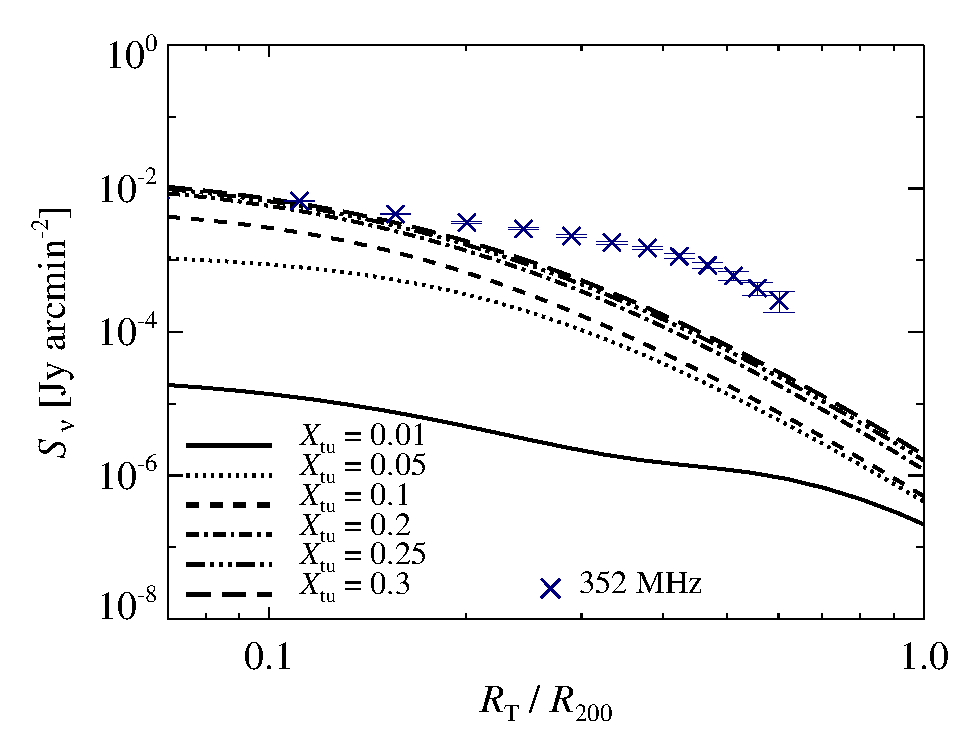
\includegraphics[width=\columnwidth]{tcltD.prof.comp.KrTTDth.Xtu.eps}
   \end{center}
\end{minipage}
\begin{minipage}{1\columnwidth}
   \begin{center}\Large{radio spectra}\\
     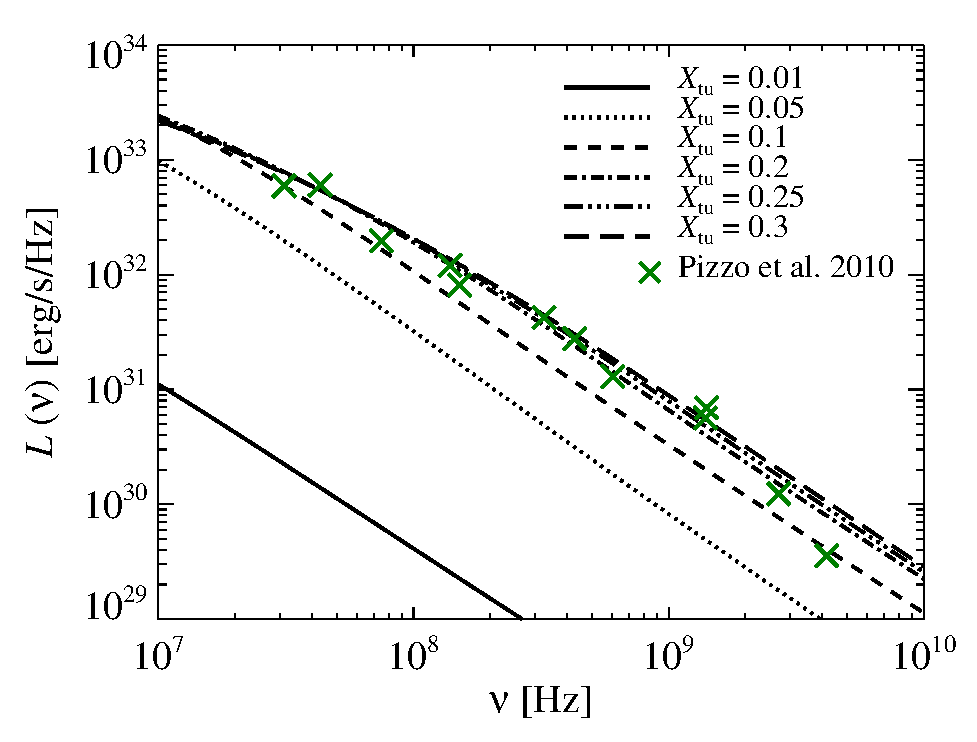
\includegraphics[width=\columnwidth]{tcltD.spec.comp.KrTTDth.Xtu.eps}
   \end{center}
\end{minipage}
\\
\begin{minipage}{1\columnwidth}
  \begin{center}%\Large{\Mflatturb:}\\ 
    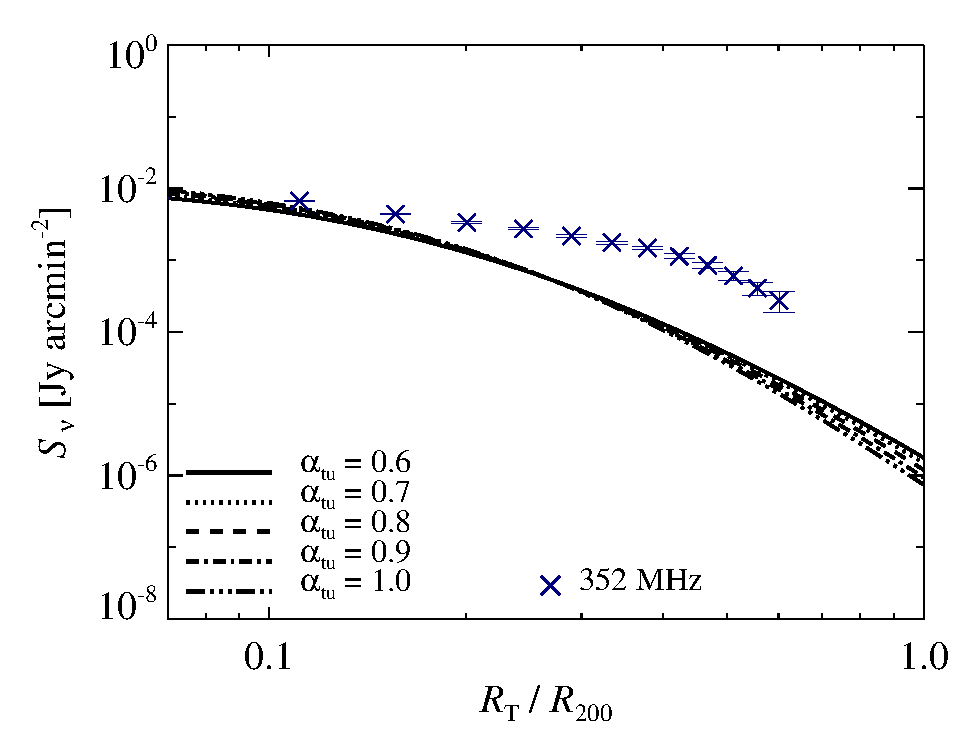
\includegraphics[width=\columnwidth]{tcltD.prof.comp.KrTTDth.aI0.eps}
  \end{center}
\end{minipage}
\begin{minipage}{1\columnwidth}
   \begin{center}%\Large{\it Brunetti et al. (2012)}:\\
     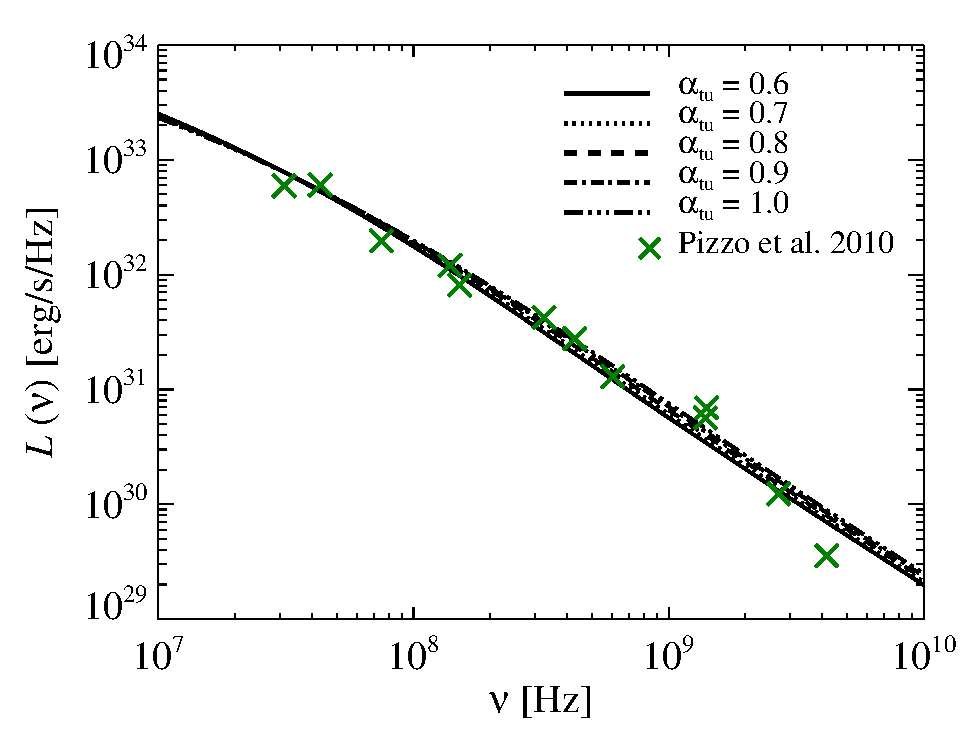
\includegraphics[width=\columnwidth]{tcltD.spec.comp.KrTTDth.aI0.eps}
   \end{center}
\end{minipage}
\\
\begin{minipage}{1\columnwidth}
  \begin{center}%\Large{\Mflatturb:}\\ 
    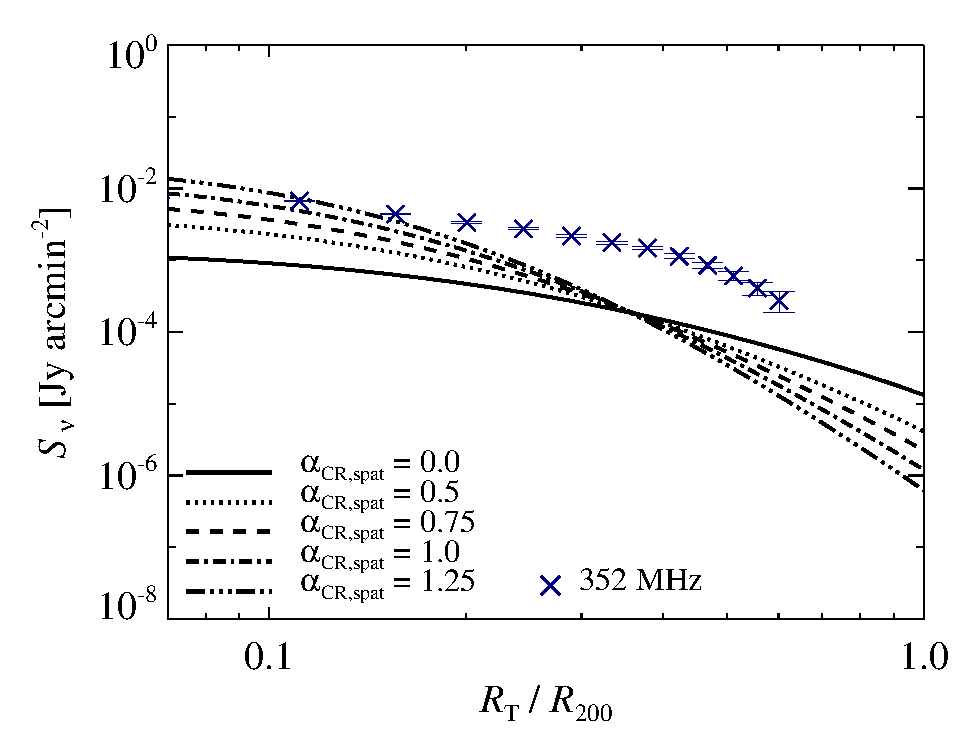
\includegraphics[width=\columnwidth]{tcltD.prof.comp.KrTTDth.aCR.eps}
  \end{center}
\end{minipage}
\begin{minipage}{1\columnwidth}
   \begin{center}%\Large{\it Brunetti et al. (2012)}:\\
     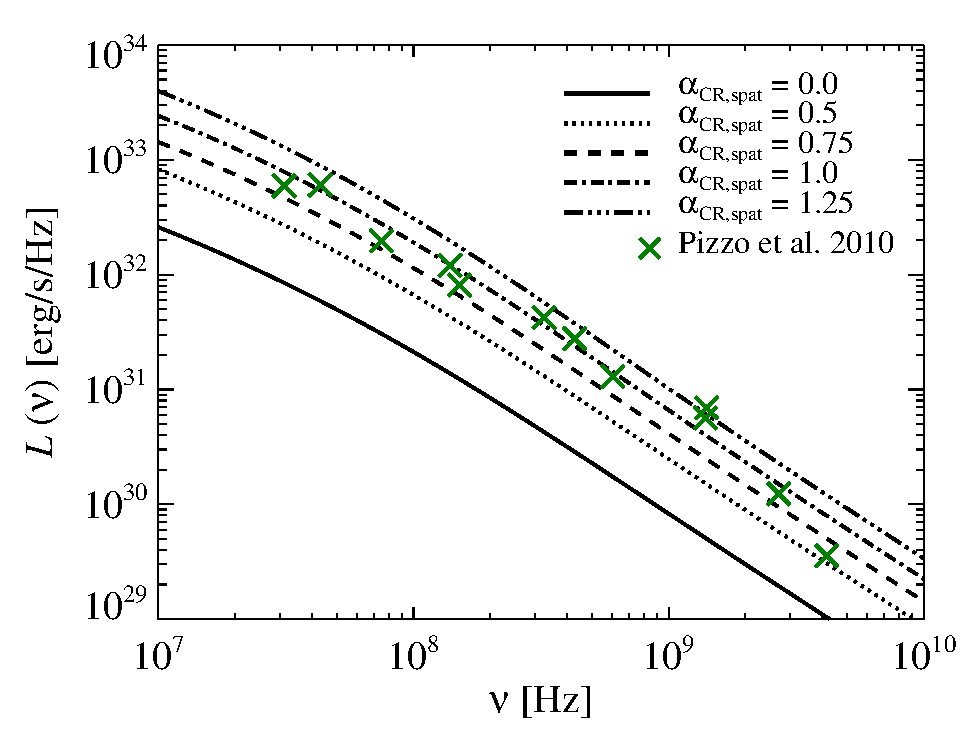
\includegraphics[width=\columnwidth]{tcltD.spec.comp.KrTTDth.aCR.eps}
   \end{center}
\end{minipage}
\caption{Sensitivity of radio emission in Coma cluster to critical
  parameters. For details see caption in
  Fig.~\ref{fig:param_comp}. For simplicity, we assume that the
  duration of reacceleration $\tau_{cl}=\tau_{\rm D}$, where $\tau_{\rm
    D}$ is the acceleration time of particles due to turbulence. In
  this scenario the radio profiles are mainly determined from the CRs,
  while the turbulence have minor impact. Interestingly, flat CR
  profiles similar to those produced through CR streaming is needed in
  order to reproduce the radio profiles.}
  \label{fig:param_comp_tcl_tD}
\end{figure*}

% --- section: Conclusions --- %
\section{Conclusions}
\label{sec:conclusions}

The standard reacceleration model for radio halos requires two ingredients with
no current direct observational constraints: a CR population which produces seed
electrons, and turbulence to perform second-order Fermi acceleration on these
electrons\footnote{Other model ingredients, such as temperature, density, and
  B-field profiles, are observationally constrained by X-ray and Faraday
  rotation measurements.}. For the best studied radio halo, Coma, there are two
main observational constraints: the radio surface brightness profile
$S_{\nu}(r)$, and the integrated luminosity as a function of frequency
$L(\nu)$. For certain assumptions about turbulence and the seed population,
analytic theoretical models can match these observations \citep{brunetti11}, but
the realism of the assumed seed electron and turbulent profiles must be
confronted with numerical simulations.

Cluster turbulence has been studied numerically in cosmological simulations with
an eye toward radio halo properties \citep{2013ApJ...771..131B,
  miniati15}, though they were not confronted against the two
benchmark observations mentioned above. Most importantly, direct simulation of the
seed electron population has been missing in the literature. In this paper, we
fill that gap. At the same time, we study the sensitivity of radio halo profiles
and spectra to variation in properties of turbulence and seed population, and
uncover the dominant effects.

In the first part of the paper, we use hydrodynamic zoom simulations of a Coma-like cluster in a cosmological setting to generate spatially and momentum-resolved seed populations of CRp's and CRe's from diffusive shock acceleration. The simulations include time-dependent cooling and adiabatic transport processes, and has been previously used in a variety of applications in CR cluster physics \citep{pinzke10,pinzke13}. The resultant CRp and CRe distribution functions then serve as initial conditions for our calculations of Fermi II acceleration by turbulence. We use time-dependent Fokker-Planck calculations which allow for spatial variations in the properties of turbulence (i.e., a spatially varying momentum diffusion coefficient). We adopt a simple parametric model for 
cluster turbulence, characterizing it by its overall normalization, spatial profile, and characteristic lifetime $\tau_{\rm cl}$. Our approach is relatively sophisticated in its treatment of the CR seed population and relatively simplified in its treatment of the turbulence; it is thus orthogonal and complementary to existing treatments which focus on the time-dependent compressible turbulence \citep{miniati15}.

Given our seed electron population (which includes both primaries generated by DSA and secondary electrons created by CRp in hadronic interactions; for standard assumptions, the latter dominates), we find that applying the standard model previously used to reproduce Coma's radio halo properties \citep{brunetti11}, in which $\eps_{\rm turb} \propto \eps_{\rm th}$, fails: it produces radio emission which is too centrally concentrated. Indeed, \citet{brunetti11} remark in their paper that the CR population required in their model is remarkably flat. By contrast, the simulations produce CRs which are more centrally concentrated.

Thus, some modification of the standard vanilla model is needed, either by modifying the spatial distribution of the CRs, or that of turbulence. We explore two examples of the former: (i) CRs can stream in the ICM, producing a flat profile \citep{ensslin11,wiener13}, or (ii) given a higher e/p ratio in DSA acceleration (perhaps due to magnetic geometry; \citealt{2014ApJ...794..153G}), the primary population can dominate. This has a much flatter profile (since secondaries must be generated collisionally, they will always be concentrated towards denser regions). However, both of these solutions still require some modification of the turbulent profile, requiring $\eps_{\rm turb}/\eps_{\rm th}$ to rise with radius. Indeed, one can simply use the unmodified CR profile derived from simulations if (iii) $\eps_{\rm turb}/\eps_{\rm th}$ rises somewhat more steeply with radius. The fact that $\eps_{\rm turb}/\eps_{\rm th}$ rises with radius is well supported by cosmological hydrodynamic simulations of clusters \citep{2009ApJ...705.1129L,2010ApJ...725.1452S,vazza11}; even the last model (iii) is (within the scatter) perfectly consistent with the trends seen by such simulations. This strongly suggests that a rising $\eps_{\rm turb}/\eps_{\rm th}$ should be part of any final model of radio halos. Given the lack of observational constraints on turbulent profiles, this unfortunately means that models will have yet another degree of freedom. 

The above models are merely meant to serve as existence proofs, showing what
modifications to the standard model are necessary to be reconciled with the
radio halo observations. There are too many uncertainties and parameter
degeneracies for any of these models to be definitive, or for one to make firm
quantitive statements about turbulent and seed CR profiles, apart from placing
certain bounds. We abstract the main parameter dependencies by exploring static,
spherically symmetric models consistent with Coma, where we repeat our
Fokker-Planck calculations. We explore three main effects: the overall
normalization of turbulence, and spatial distribution of turbulence and cosmic
rays.

We find that the most important variable is the overall normalization of
turbulence: surface brightness scales exponentially with the amount of
turbulence. The radio spectrum also becomes more curved with higher
turbulence. In contrast, the surface brightness scales linearly with the CR
abundance.  The spatial distribution of both turbulence and CRs also influence
radio halos profiles (for both, flatter distributions at fixed overall
normalization imply flatter surface brightness profiles with lower overall radio
luminosity), but play a secondary role.

This exponential dependence of radio halo luminosity with turbulence then raises
the interesting question of why radio halo scaling relations (e.g.,
$L_{\nu}$--$L_{\rm X}$) are so tight. Previous statistical modeling of radio
halo populations \citep{2006MNRAS.369.1577C,2007MNRAS.378.1565C} have focused
on matching the mean relations, but not the scatter. We believe the latter
provides a particularly interesting and potentially fruitful constraint. The
acceleration timescale $\tau_{\rm D}$ and the length of time during which
acceleration takes place $\tau_{\rm cl}$ must be matched so that there are
roughly $\sim 2$ e-folds (given the factor $\sim 10$ difference in radio
luminosity between the radio bright and faint populations; \citet{brown11}),
otherwise scatter in turbulence (which we might expect given the wide variety of
merger and infall conditions) will be exponentially amplified in radio
luminosity. The timescale of the merger has some natural scatter which is not
obviously correlated with $\tau_{\rm D}$. 

If instead we adopt $\tau_{\rm
  cl} \sim \tau_{\rm decay}$, i.e. the natural lifetime of turbulence is its decay lifetime, then we can show that the acceleration time and the lifetime of turbulence are linked, simply because the wave-particle interaction rate (which drives particle acceleration) and the wave-wave interaction rate (which drives dissipation) are linked. If we are mindful that Kraichnan turbulence is only applicable below the Alfven scale $l_{\rm A}$ (where turbulent velocities $v < v_{\rm A}$), then remarkably the ratio $\tau_{\rm cl}/\tau_{\rm D}$ is independent of properties of the turbulence (such as its amplitude and outer scale) and only depends on plasma parameters. Our results suggest that TTD on thermal particles may result in overly rapid damping of turbulence, and inefficient acceleration (equation \ref{eqn:ratios_TTD}), but if plasma instabilities scatter the thermal particles so that the fast modes damp via TTD on the cosmic rays, then the required acceleration can take place (equation \ref{eqn:ratios_CR_damp}). In agreement with other assessments, we find that if turbulence is Burgers rather than Kraichnan, then turbulent reacceleration is ineffective, and some other explanation for radio halos (e.g., magnetic reconnection, \cite{brunetti16}) is necessary. If we adopt the ansatz $\tau_{\rm cl} \sim \tau_{\rm D}$, then we find that above a threshold level of turbulence (necessary to overcome cooling), radio properties are insensitive to both the amplitude and spatial profile of turbulence, since only a fixed, asymptotic amount of amplification takes place. On the other hand, they {\it are} sensitive to the properties of the seed electron profile. This raises the exciting possibility that one could marginalize over the highly uncertain properties of cluster turbulence to learn about the underlying seed CR population. Our results suggest that studying not just mean trends, but the relatively small scatter in radio-halo scaling relations, may prove extremely fruitful in shedding light on ICM plasma processes. 


{\bf Acknowledgments.} We thank Josh Wiener for discussions on CR streaming,
Lawrence Rudnick for discussion on uncertainties in the 1.4 GHz radio data,
Fabio Zandanel for re-calculating gamma-ray limits, and Gianfranco Brunetti for
useful discussions. We thank an anonymous referee for helpful comments that
improved the paper. A.P. is grateful to the Swedish research council for
financial support. S.P.O. thanks NASA grants NNX12AG73G and NNX15AK81G for
support, as well as KITP for hospitality. This research was supported in part by
the National Science Foundation under Grant No. NSF
PHY11-25915. C.P.~acknowledges support by the European Research Council under
ERC-CoG grant CRAGSMAN-646955 and by the Klaus Tschira Foundation.


%%%%%%%%%%%%%%%%%%%%%%%%%%%%%%%%%%%%%%%%%%%%%%%%%%%%%%%%%%%%%%%
\vspace{-0.7cm}

\bibliography{paper}
\bibliographystyle{mnras}

\end{document}
